%%----------------------------------------------------------------------------------------
\clearpage
\pagestyle{fancy}
%%----------------------------------------------------------------------------------------
%%       PREFAZIONE
%%----------------------------------------------------------------------------------------
\part{Una valida alternativa per calcolare $N$, $T$ ed $M$}
\setcounter{section}{0}
%----------------------------------------------------------------------------------------
Facciamo ancora riferimento alla figura~\vref{figura11-1} e supponiamo di voler calcolare $N$, $T$ ed $M$ nella sezione $\mathcal{S}$. Nulla vieta di interpretare $\mathcal{S}$ come un \textsc{incastro interno} che salda le parti $A\mathcal{S}$ ed $\mathcal{S}D$. Risulta ovvio che, se si tagliasse in corrispondenza di $\mathcal{S}$, le parti $A\mathcal{S}$ ed $\mathcal{S}D$ non starebbero più in equilibrio; se però, in $\mathcal{S}$ si facessero agire le reazioni dell'incastro interno, due forze ed un momento, allora l'equilibrio sarebbe ripristinato. In figura~\ref{figura12-1} abbiamo disegnato le parti $A\mathcal{S}$ ed $\mathcal{S}D$ ed in $\mathcal{S}$ abbiamo segnato le reazioni dell'incastro su entrambe le parti. 
%----------------------------------------------------------------------------------------
%--------------------------------------------------------------------------------------------------------------------------------------------------------------
\renewcommand{\thefigure}{12~-~1}
\begin{figure}[ht]
\centering
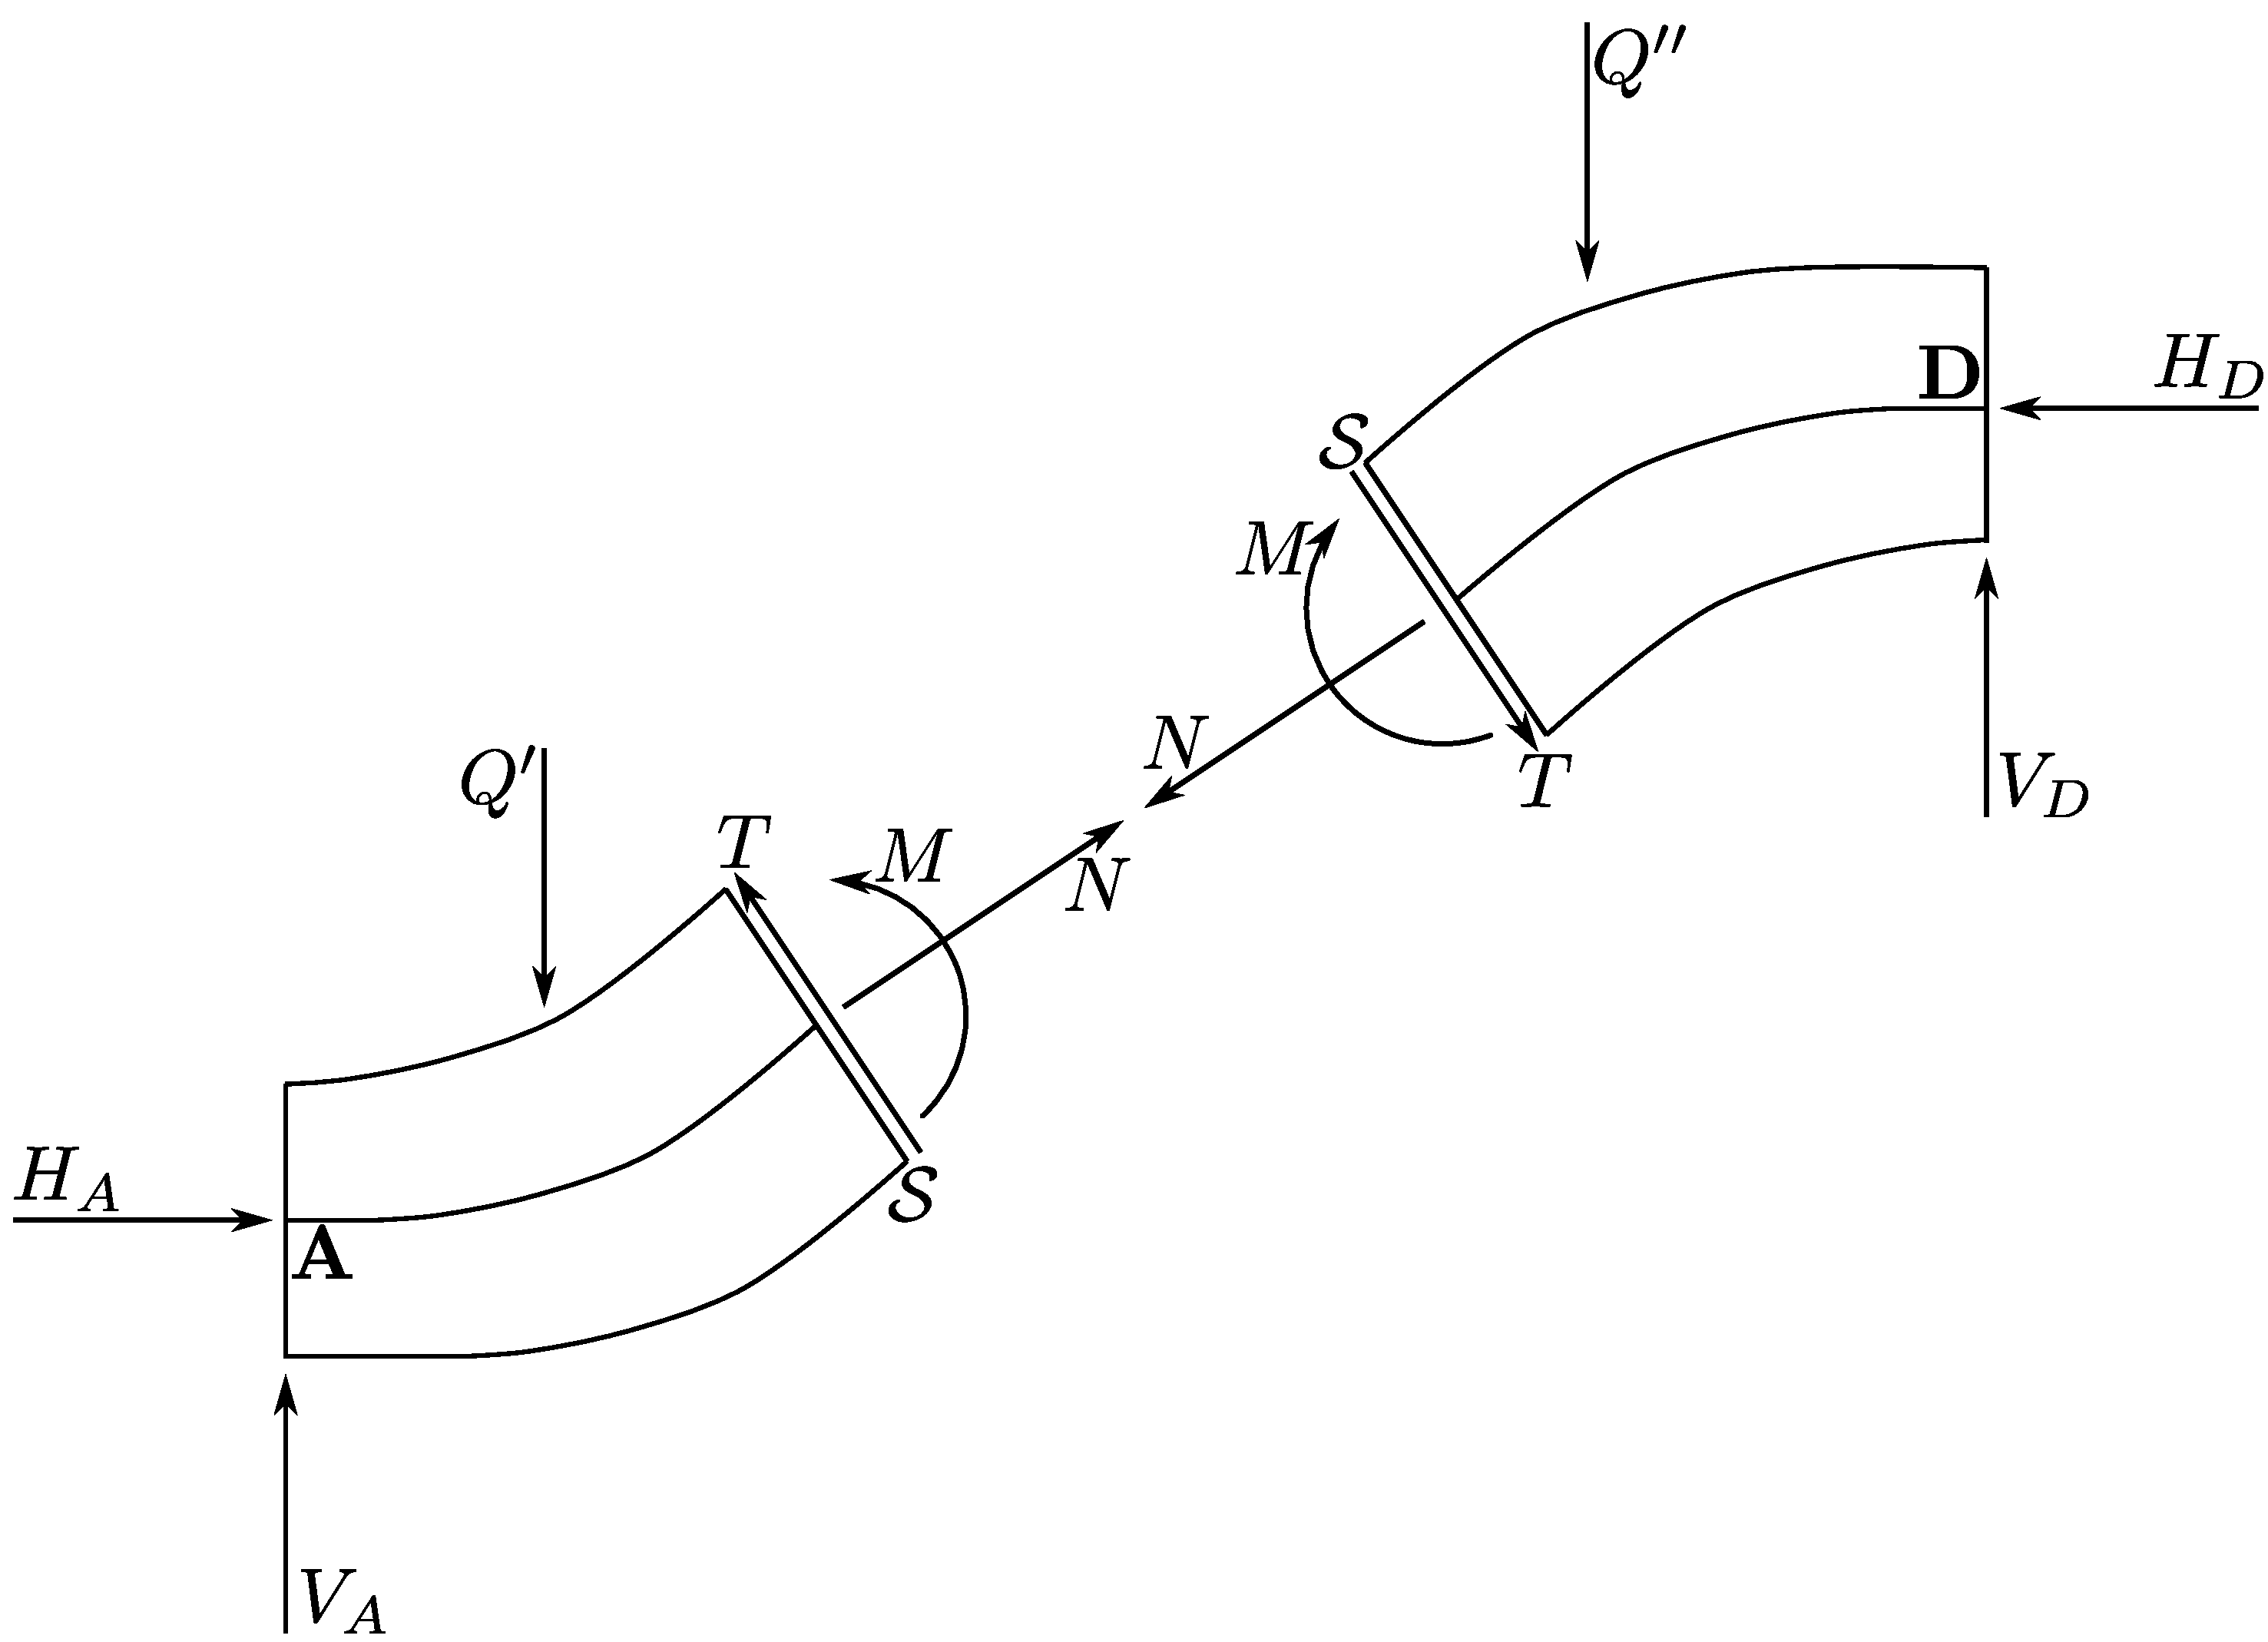
\includegraphics[width=0.89\textwidth]{Immagini/Parte_12/Figura12_1/figura12_1.pdf}
\caption{}
\label{figura12-1}
\end{figure}
%--------------------------------------------------------------------------------------------------------------------------------------------------------------
%----------------------------------------------------------------------------------------
L'incastro interno, come pure quello esterno, reagisce, come è noto, con un momento ed una forza comunque diretta; quest'ultima può essere scomposta lungo le direzioni individuate dalle rette $n$ e $t$; in tal modo, le reazioni dell'incastro interno $\mathcal{S}$ si identificano con le caratteristiche della sollecitazione in $\mathcal{S}$. In figura~\ref{figura12-1} sono visibili
%----------------------------------------------------------------------------------------
\begin{enumerate}
\item le reazioni dell'incastro $\mathcal{S}$ sulla parte $A\mathcal{S}$; sarebbe più preciso affermare che sono visibili le azioni che la parte $\mathcal{S}D$ esercita attraverso la sezione $\mathcal{S}$ sulla parte $A\mathcal{S}$;
\item le azioni che la parte $A\mathcal{S}$ esercita attraverso la sezione $\mathcal{S}$ sulla parte $\mathcal{S}D$.
\end{enumerate}
%----------------------------------------------------------------------------------------
Vogliamo sottolineare che in figura~\ref{figura12-1} si sono segnati $M$, $N$ e $T$ col \textsc{verso positivo}; questa affermazione trova conferma nelle stesse definizioni di $M$, $N$ e $T$ date nel paragrafo precedente. Essendo in equilibrio la parte $A\mathcal{S}$, saranno verificate le tre equazioni:
%----------------------------------------------------------------------------------------
\begin{equation} \label{equazione12-1}
\boxed{ \text{Traslazione lungo } n} \,\, \longrightarrow \,\, N+H_{A}\cdot \cos{\alpha} + V_{A}\cdot \sin{\alpha} - Q' \cdot \sin{\alpha} = 0 \tag{12.1}
\end{equation}
%----------------------------------------------------------------------------------------
Dall'equazione~\eqref{equazione12-1} si perviene alla stessa espressione di $N$ che si era trovata nel paragrafo precedente, considerando le forze che precedono $\mathcal{S}$, come si può osservare andando ad esaminare le componenti esplicitate nel paragrafo precedente. 
%----------------------------------------------------------------------------------------
\begin{equation} \label{equazione12-2}
\boxed{ \text{Traslazione lungo } t} \,\, \longrightarrow \,\, T - H_{A}\cdot \sin{\alpha} + V_{A}\cdot \cos{\alpha} - Q'\cdot \cos{\alpha} = 0 \tag{12.2}
\end{equation}
%----------------------------------------------------------------------------------------
Dall'equazione~\eqref{equazione12-2} si perviene alla stessa espressione di $T$ che si era trovata nel paragrafo precedente, considerando le forze che precedono $\mathcal{S}$. 
%----------------------------------------------------------------------------------------
\begin{equation} \label{equazione12-3}
\boxed{ \text{Rotazione (polo nel baricentro di } \mathcal{S})} \,\, \longrightarrow \,\, M + H_{A}\cdot b_{1} - V_{A}\cdot b_{2} + Q'\cdot b_{3} = 0 \tag{12.3}
\end{equation}
%----------------------------------------------------------------------------------------
%----------------------------------------------------------------------------------------
Dall'equazione~\eqref{equazione12-3} si perviene alla stessa espressione di $M$ che si era trovata nel paragrafo precedente, considerando le forze che precedono $\mathcal{S}$. In maniera analoga, è possibile esprimere $M$, $N$ e $T$ in $\mathcal{S}$ scrivendo le equazioni di equilibrio della parte $\mathcal{S}D$. 
%----------------------------------------------------------------------------------------
\section{Sollecitazione interna vista sul concio}
%----------------------------------------------------------------------------------------
%--------------------------------------------------------------------------------------------------------------------------------------------------------------
\renewcommand{\thefigure}{12~-~2}
\begin{figure}[ht]
\centering
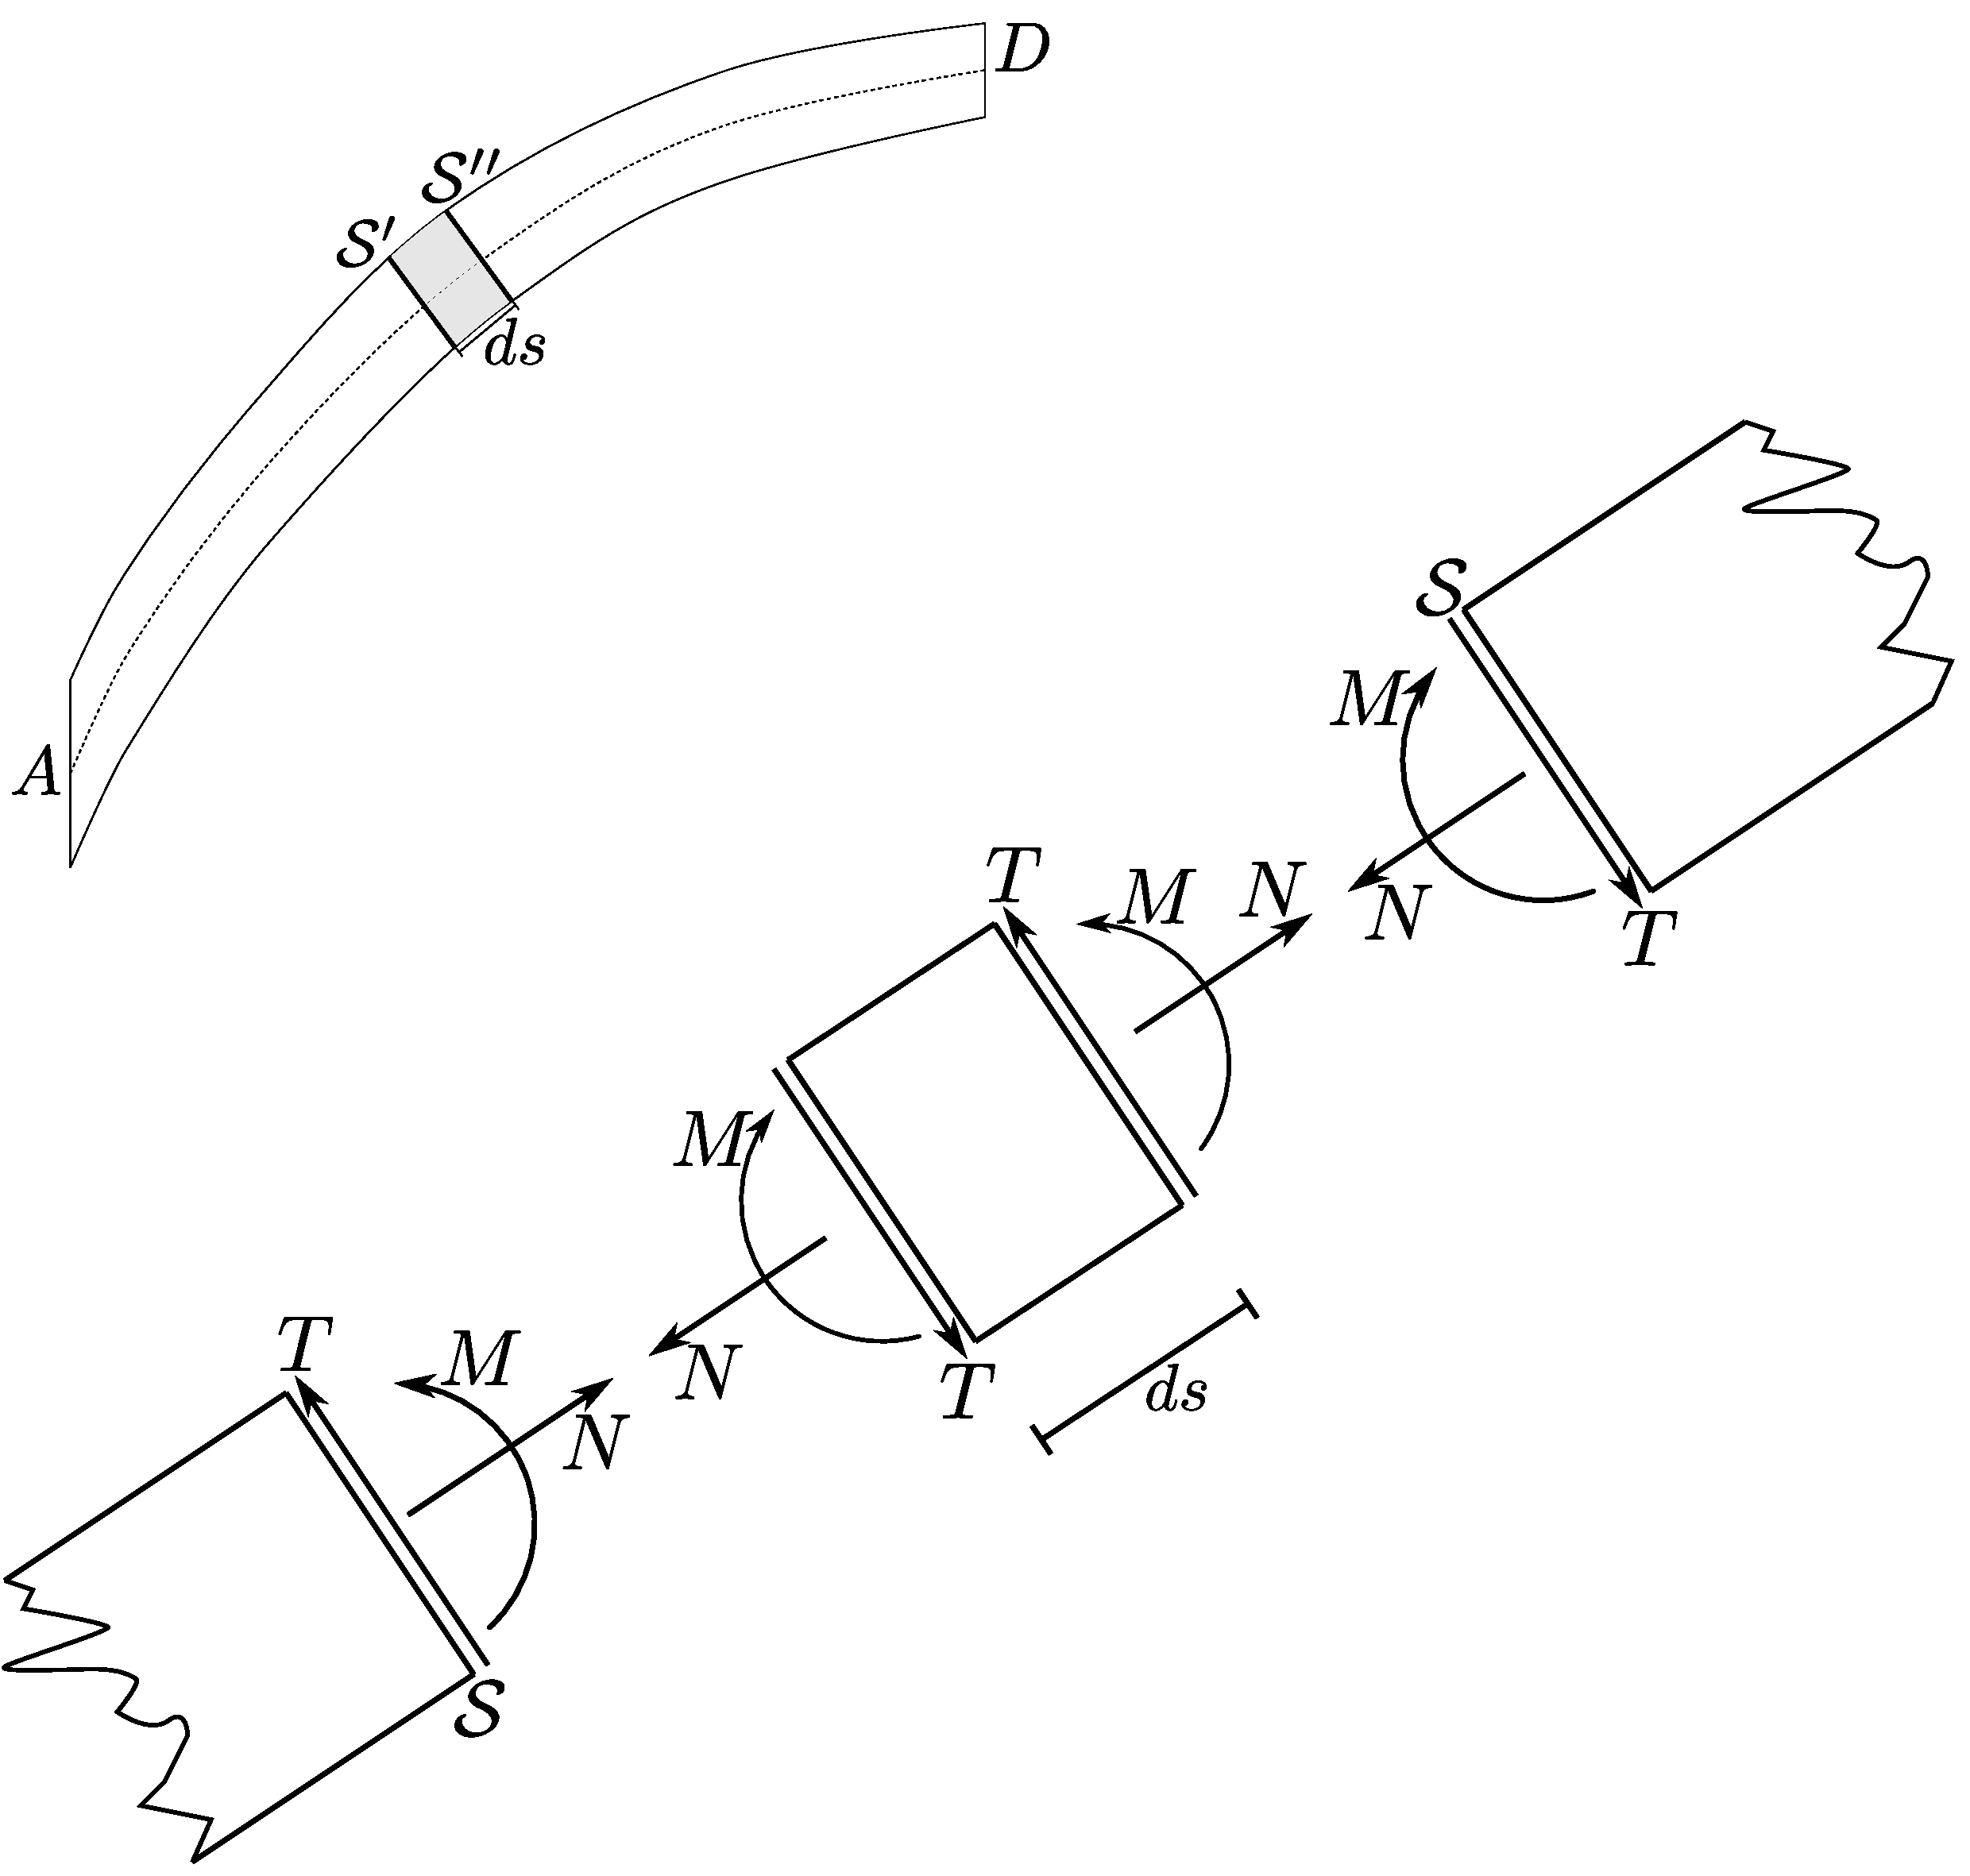
\includegraphics[width=0.68\textwidth]{Immagini/Parte_12/Figura12_2/figura12_2.pdf}
\caption{}
\label{figura12-2}
\end{figure}
%--------------------------------------------------------------------------------------------------------------------------------------------------------------
Ogni trave può intendersi come un assemblaggio di infiniti \textsc{conci}, cioè di \emph{fettine} di spessore infinitesimo $ds$, incastrate le une alle altre. In figura~\ref{figura12-2} è evidenziato il concio che si trova \emph{a cavallo} della sezione $\mathcal{S}$; abbiamo indicato con $\mathcal{S}'$ ed $\mathcal{S}''$ le due sezioni che lo delimitano. Esso può intendersi, ovviamente, come un \textsc{giunto} che rende solidali le parti $A\mathcal{S}'$ ed $\mathcal{S}''D$. Le facce $\mathcal{S}'$ ed $\mathcal{S}''$ possono intendersi come \textsc{incastri interni} fra il giunto e le due parti $A\mathcal{S}'$ ed $\mathcal{S}''D$; identificando le reazioni dell'incastro interno con le sollecitazioni, abbiamo un'altra maniera di visualizzare $M$, $N$ e $T$; si osservi con attenzione la figura~\ref{figura12-2}, dove i versi di $M$, $N$ e $T$ sono chiaramente quelli positivi.
%--------------------------------------------------------------------------------------------------------------------------------------------------------------
\renewcommand{\thefigure}{12~-~3}
\begin{figure}[ht]
\centering
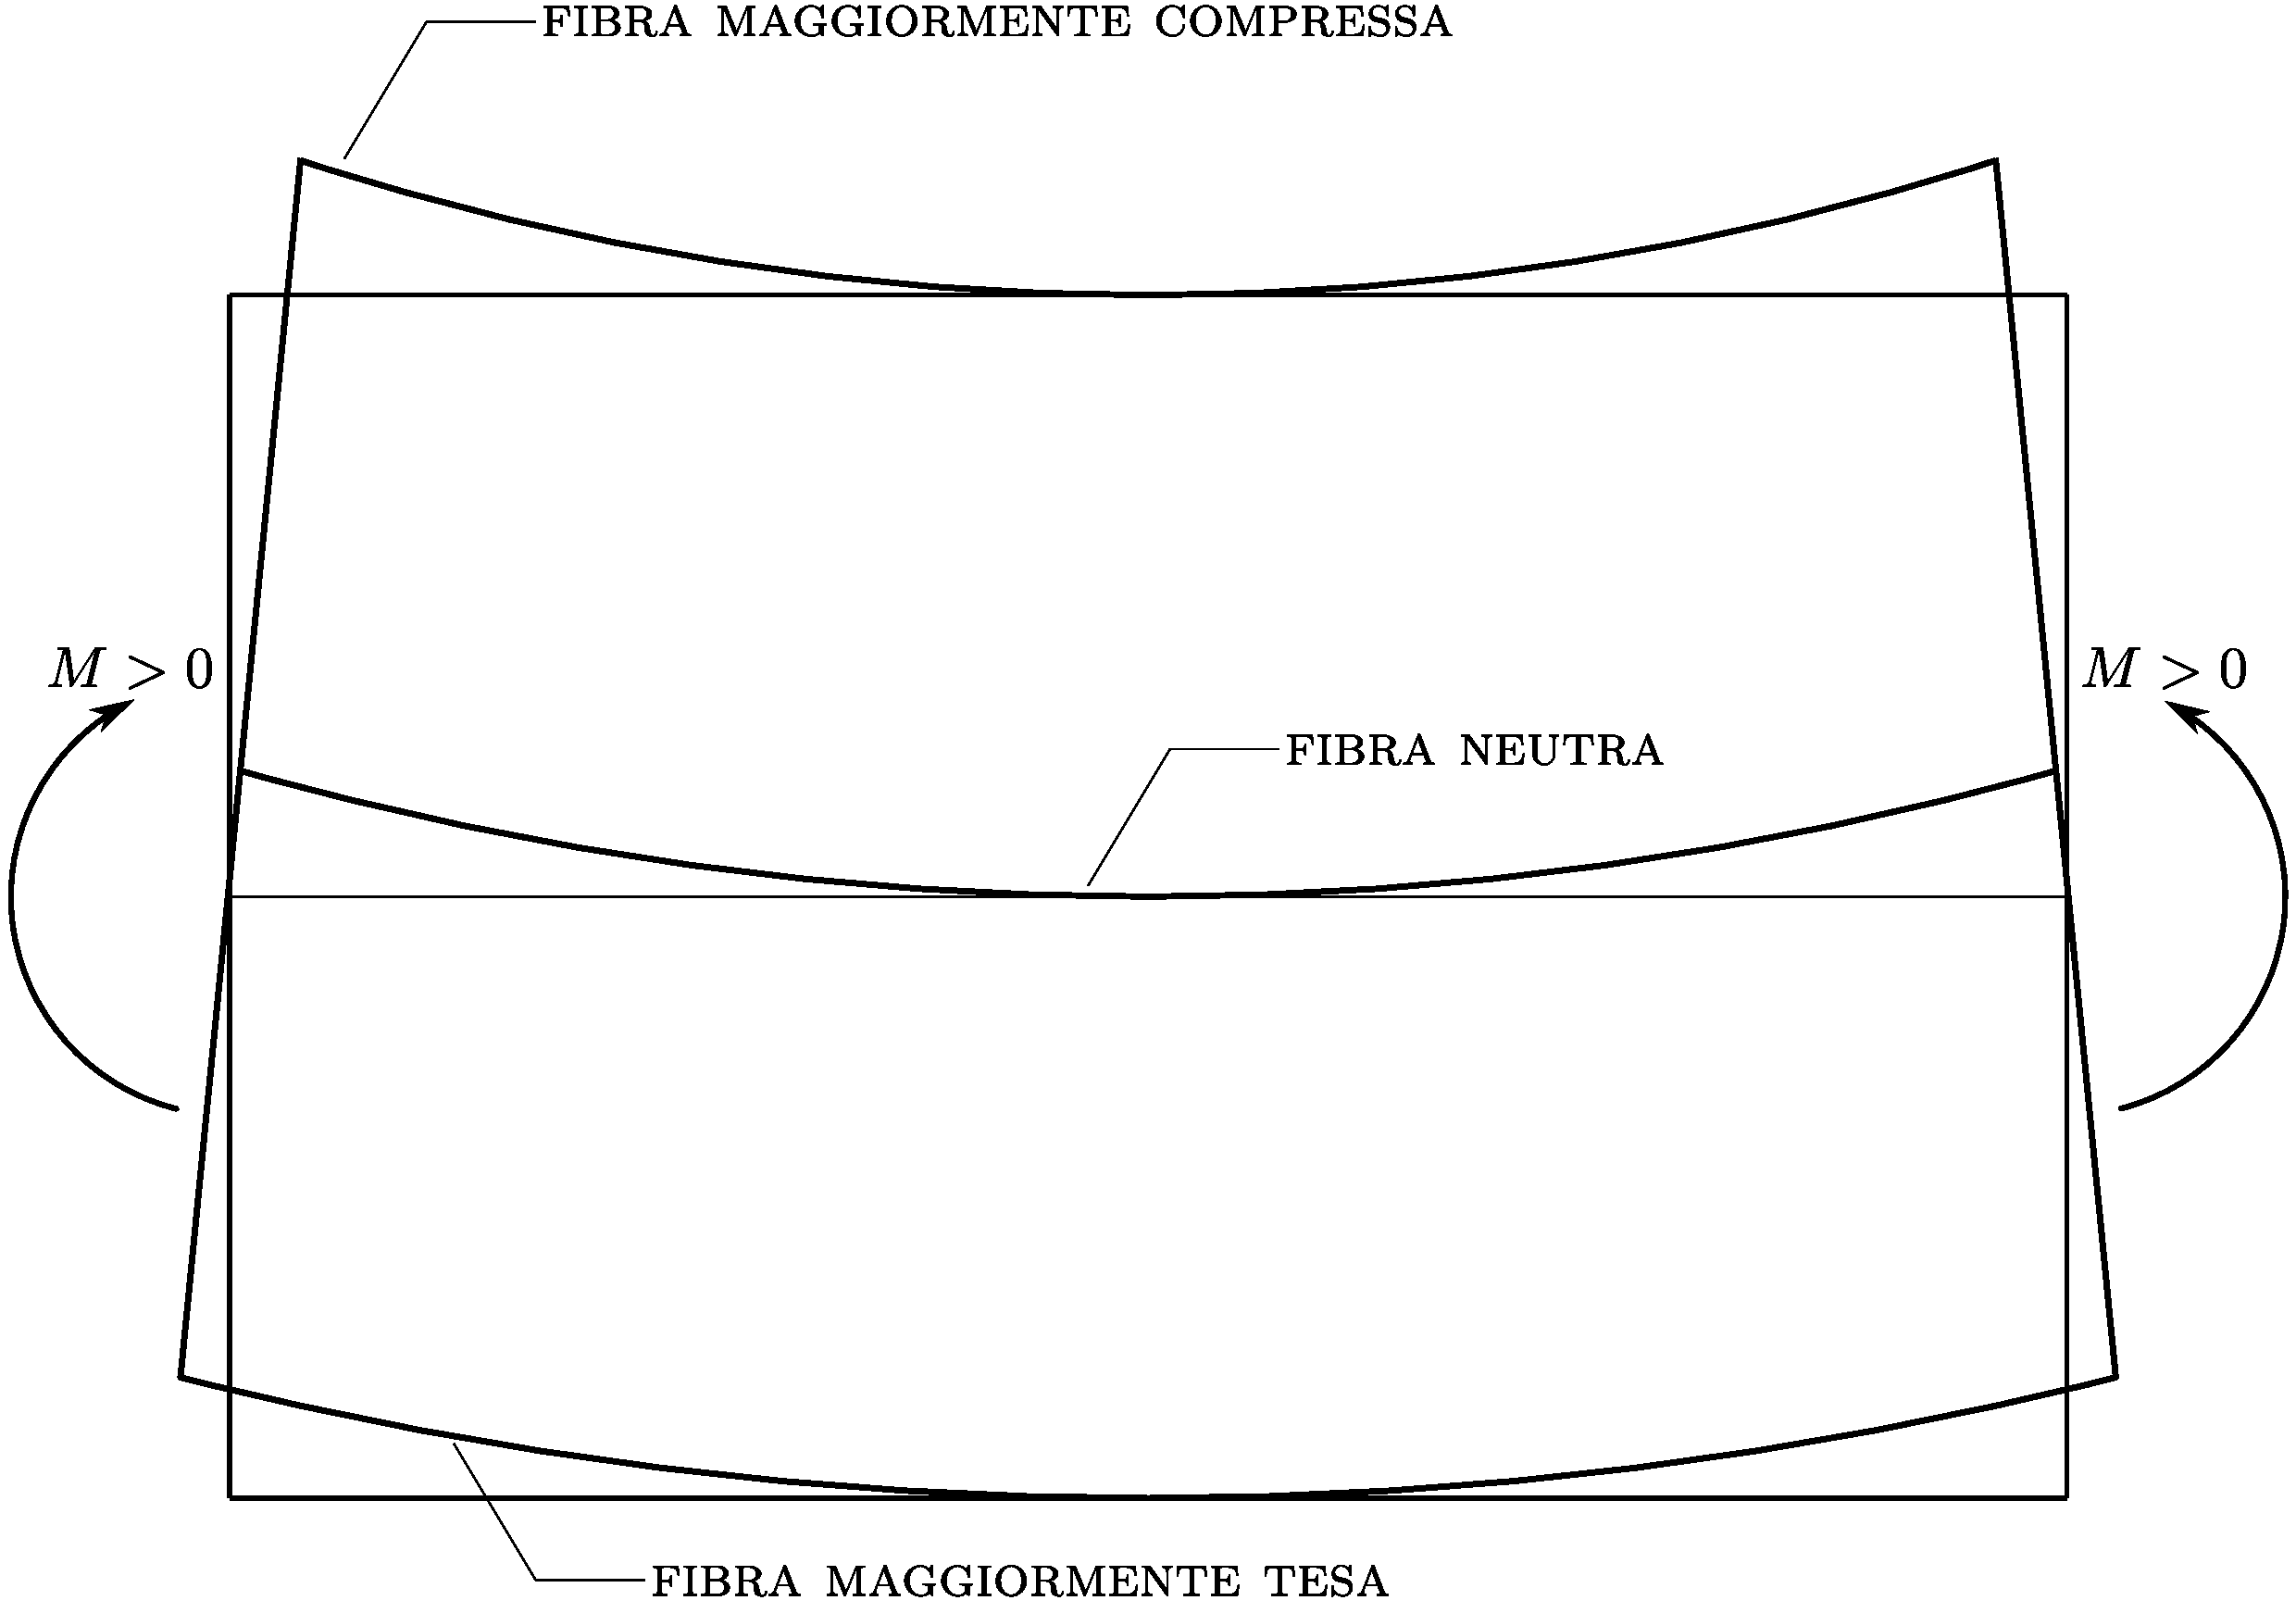
\includegraphics[width=0.58\textwidth]{Immagini/Parte_12/Figura12_3/figura12_3.pdf}
\caption{}
\label{figura12-3}
\end{figure}
%--------------------------------------------------------------------------------------------------------------------------------------------------------------
A proposito di $M$, vale la pena osservare che, se il concio fosse di materiale deformabile, si pensi ad esempio alla gomma, un momento positivo gli farebbe assumere la configurazione visibile in figura~\ref{figura12-3}; quest circostanza si esprime dicendo che un momento positivo \textbf{\textsc{tende le fibre inferiori}}. La locuzione \emph{tende le fibre inferiori} calza quando il verso di percorrenza di $s$ è da sinistra a destra, come nel caso della nostra figura. In situazioni diverse, risulta più corretto affermare quando segue:
%--------------------------------------------------------------------------------------------------------------------------------------------------------------
\\

\fbox{\begin{minipage}{38em}
\centering
\textsc{Il momento $M$ risulta positivo se tende le fibre a destra di un osservatore che si muova nel verso delle $s$ crescenti.}
\end{minipage}}\\
%--------------------------------------------------------------------------------------------------------------------------------------------------------------
\section{Sollecitazione interna e carichi ripartiti nelle travi}
%----------------------------------------------------------------------------------------
%--------------------------------------------------------------------------------------------------------------------------------------------------------------
\renewcommand{\thefigure}{12~-~4}
\begin{figure}[ht]
\centering
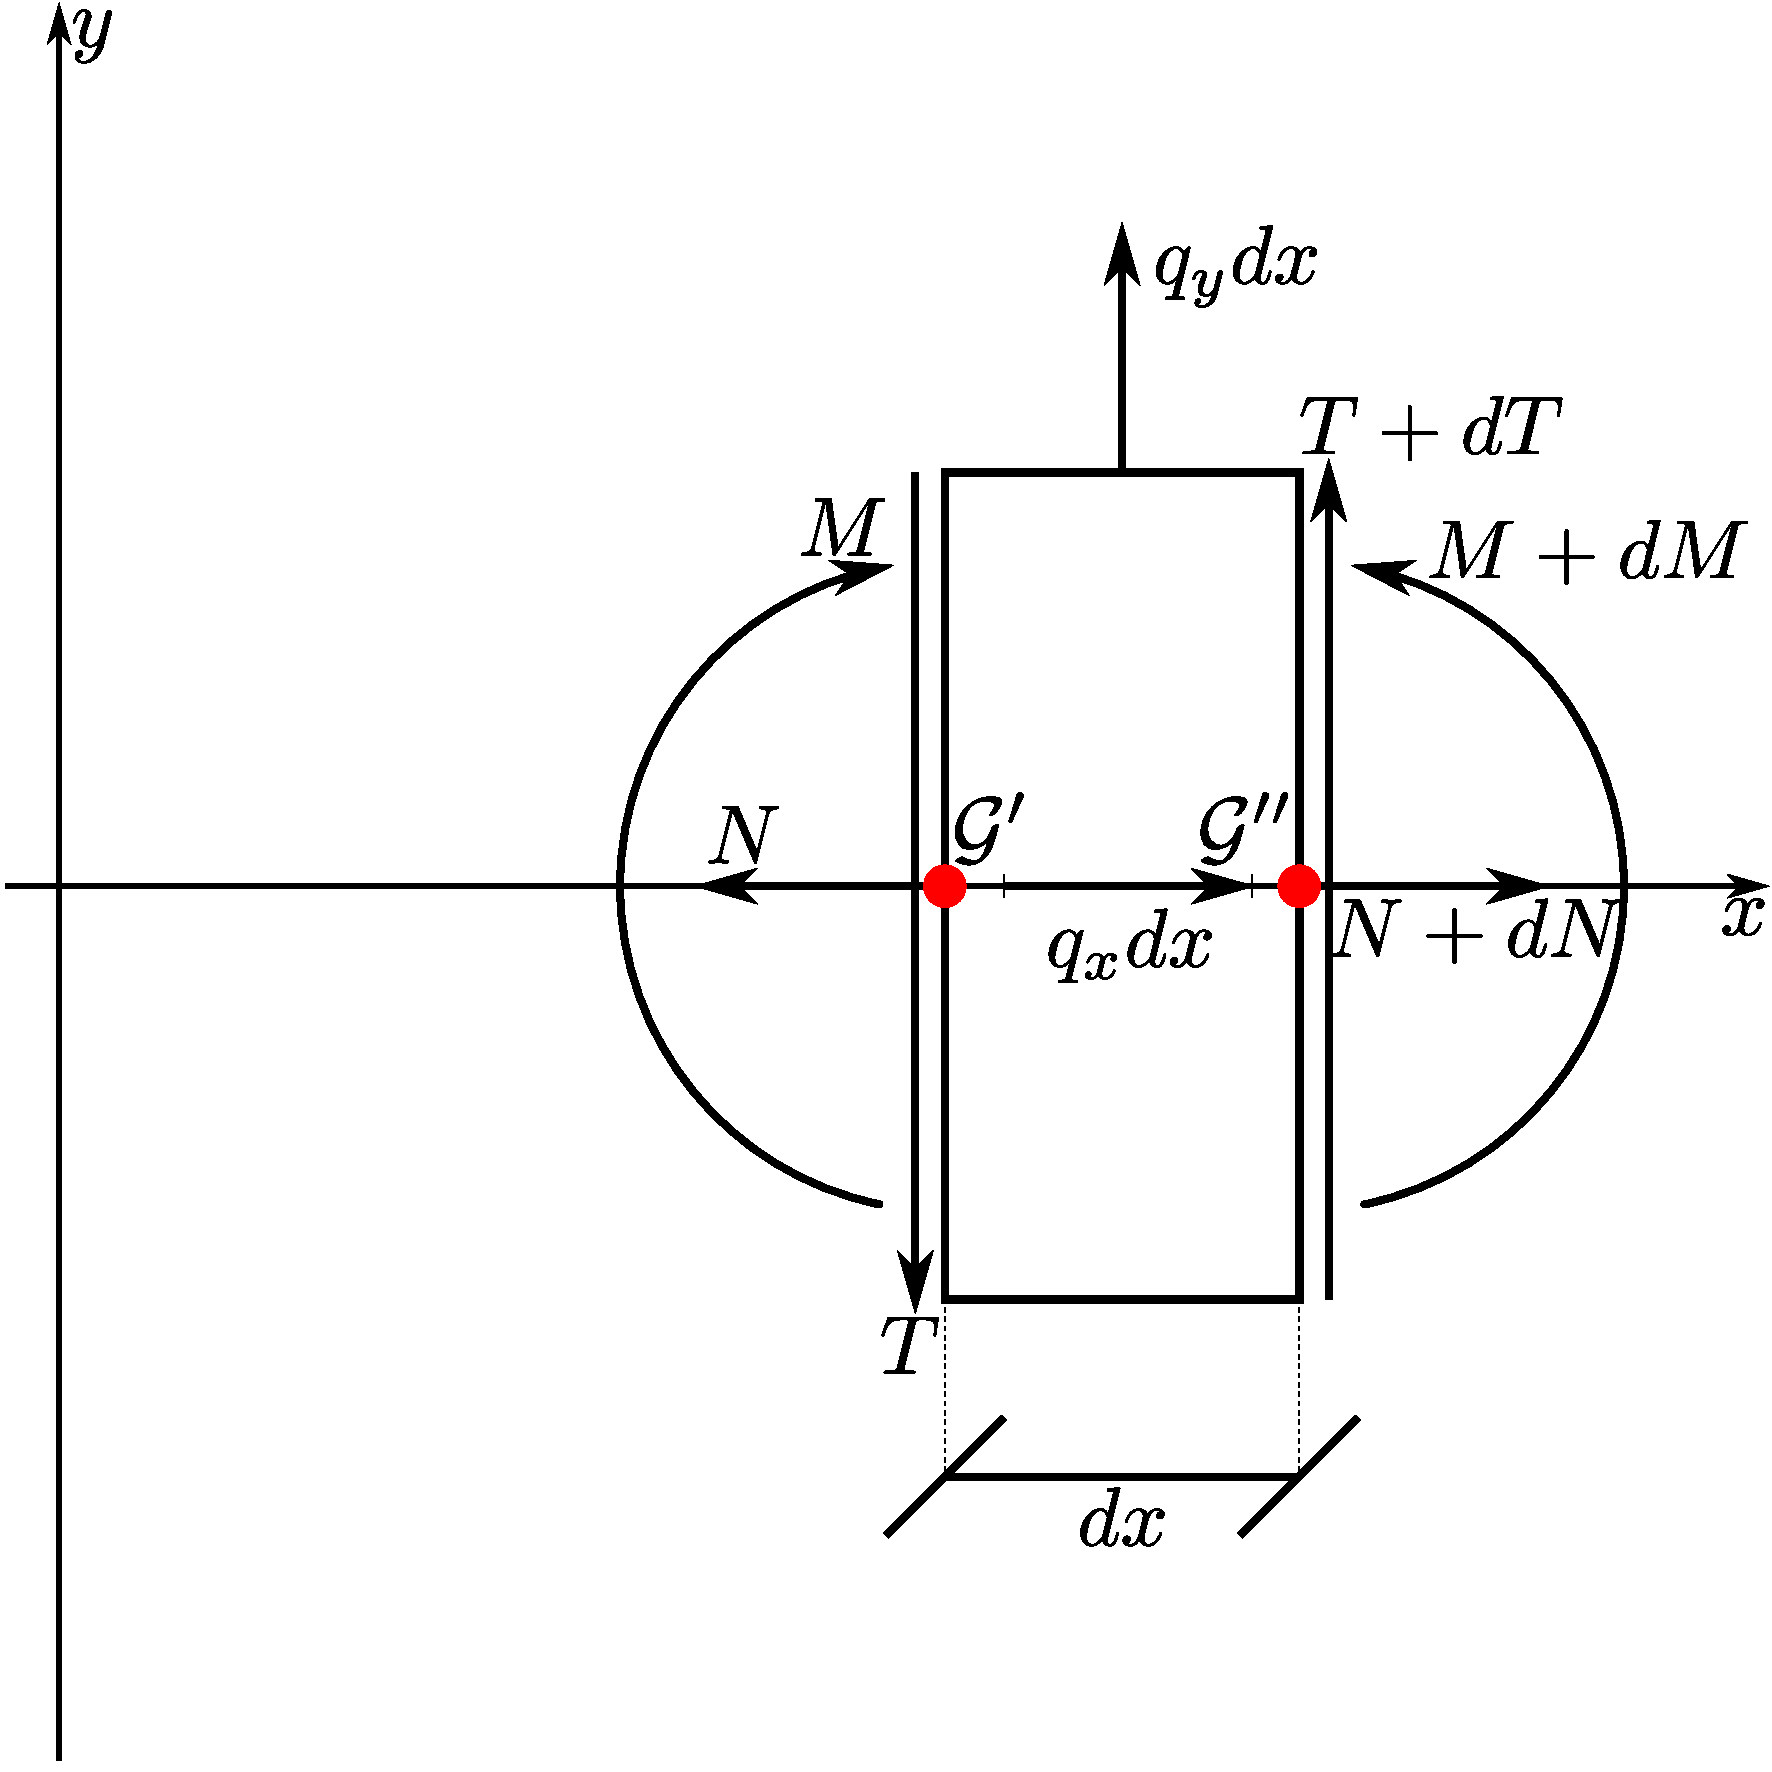
\includegraphics[width=0.562\textwidth]{Immagini/Parte_12/Figura12_4/figura12_4.pdf}
\caption{}
\label{figura12-4}
\end{figure}
%--------------------------------------------------------------------------------------------------------------------------------------------------------------
In figura~\ref{figura12-4} è rappresentato un concio di trave rettilinea; su di esso, nel caso più generale, agiscono le forze elementari dovute ai carichi distribuiti: $q_{x}dx$ e $q_{y}dy$, che sono positivi così come rappresentati in figura. Si sono anche segnate, sempre col verso positivo, le caratteristiche della sollecitazione; sulla faccia sinistra del concio esse valgono $M$, $N$ e $T$; sulla faccia destra, trattandosi di funzioni di $x$, esse risultano incrementate e valgono rispettivamente $N+dN$, $M+dM$ e $T+dT$. Poiché la trave è in equilibrio, dovrà esere in equilibrio ogni suo concio; scriviamo dunque, per il concio rappresentato in figura~\ref{figura12-4}, le tre seguenti equazioni:
%----------------------------------------------------------------------------------------
\begin{subequations}
\begin{align} 
- N + q_{x}dx + N + dN &= 0 \quad [\rightarrow] \label{equazione12-4a} \tag{12.4a} \\
- T + q_{y}dy + T + dT &= 0 \quad [\uparrow] \label{equazione12-4b} \tag{12.4b} \\
- M + M + dM + T\cdot dx - q_{y}\frac{dx^2}{2} &= 0 \quad [G'\,\, \circlearrowleft] \label{equazione12-4c} \tag{12.4c} \\
\end{align}
\end{subequations}
%----------------------------------------------------------------------------------------
dove con $G'$ si è indicato il baricentro della sezione $\mathcal{S}'$. Semplificando le relazioni precedenti, si ottiene quanto segue; si noti che nell'equazione di equilibrio alla rotazione rispetto al polo $G'$ si considera il termine $q_{y}\frac{dx^2}{2}$ un \textbf{infinitesimo di ordine superiore} e, dunque, trascurabile rispetto agli altri termini:
%----------------------------------------------------------------------------------------
\begin{subequations}
\begin{align} 
q_{x}dx + dN &= 0 \label{equazione12-5a} \tag{12.5a} \\
q_{y}dy + dT &= 0 \label{equazione12-5b} \tag{12.5b} \\
dM + T\cdot dx &= 0 \label{equazione12-5c} \tag{12.5c} \\
\end{align}
\end{subequations}
%----------------------------------------------------------------------------------------
Per cui, in definitiva, dalle relazioni~\eqref{equazione12-5a},~\eqref{equazione12-5b} e~\eqref{equazione12-5c} ricaviamo:
%--------------------------------------------------------------------------------------------------------------------------------------------------------------
\\

\fbox{\begin{minipage}{38em}
\centering
\begin{equation} \label{equazione12-6}
\frac{dN}{dx} = -q_{x} \,\, \longrightarrow \,\, N = - \int q_{x}\,dx + c_1 \tag{12.6}
\end{equation}
\end{minipage}}\\
%--------------------------------------------------------------------------------------------------------------------------------------------------------------
%--------------------------------------------------------------------------------------------------------------------------------------------------------------
\\

\fbox{\begin{minipage}{38em}
\centering
\begin{equation} \label{equazione12-7}
\frac{dT}{dx} = -q_{y} \,\, \longrightarrow \,\, T = - \int q_{y}\,dx + c_2 \tag{12.7}
\end{equation}
\end{minipage}}\\
%--------------------------------------------------------------------------------------------------------------------------------------------------------------
%--------------------------------------------------------------------------------------------------------------------------------------------------------------
\\

\fbox{\begin{minipage}{38em}
\centering
\begin{equation} \label{equazione12-8}
\frac{dM}{dx} = -T \,\, \longrightarrow \,\, M = - \int T\,dx + c_3 \tag{12.8}
\end{equation}
\end{minipage}}\\
%--------------------------------------------------------------------------------------------------------------------------------------------------------------

\noindent Le costanti di integrazione $c_1$, $c_2$ e $c_3$ si ricavano, ovviamente, imponendo le condizioni ai limiti. Le relazioni~\eqref{equazione12-6},~\eqref{equazione12-7} e~\eqref{equazione12-8} fanno da supporto alle seguenti, notevoli proposizioni:
%----------------------------------------------------------------------------------------
%--------------------------------------------------------------------------------------------------------------------------------------------------------------
\begin{prop}
Su un tratto rettilineo su cui non c'è un carico assiale distribuito ($q_{x} = 0 $) risulta 
\begin{equation*}
N = \text{Funzione costante}
\end{equation*}
\end{prop}
%----------------------------------------------------------------------------------------
\begin{prop}
Su un tratto rettilineo su cui c'è un carico assiale uniformemente distribuito ($q_{x} = \text{costante}$) risulta 
\begin{equation*}
N = \text{Funzione lineare}
\end{equation*}
\end{prop}
%----------------------------------------------------------------------------------------
\begin{prop}
Su un tratto rettilineo su cui agisce un $q_{x} = \text{Funzione polinomiale di grado } n$ risulta 
\begin{equation*}
N = \text{Funzione polinomiale di grado } n+1
\end{equation*}
\end{prop}
%----------------------------------------------------------------------------------------
\begin{prop}
Su un tratto rettilineo su cui non c'è un carico trasversale distribuito ($q_{y} = 0$) risulta 
\begin{align*}
T &= \text{Funzione costante} \\ 
M &= \text{Funzione lineare} 
\end{align*}
Nulla esclude il caso in cui $T=0$ ed $M=\text{costante}$.
\end{prop}
%----------------------------------------------------------------------------------------
\begin{prop}
Su un tratto rettilineo su cui c'è un carico trasversale uniformemente distribuito ($q_{y} = \text{costante}$) risulta 
\begin{align*}
T &= \text{Funzione lineare} \\ 
M &= \text{Funzione quadratica}
\end{align*}
\end{prop}
%----------------------------------------------------------------------------------------
\begin{prop}
Su un tratto rettilineo su cui c'è un $q_{y} = \text{Funzione polinomiale di grado } n$ risulta 
\begin{align*}
T &= \text{Funzione polinomiale di grado } n+1 \\ 
M &= \text{Funzione polinomiale di grado } n+2
\end{align*}
\end{prop}
%--------------------------------------------------------------------------------------------------------------------------------------------------------------
\clearpage
\section{Esercizi}
\paragraph{Esercizio 12.1}
%--------------------------------------------------------------------------------------------------------------------------------------------------------------
\renewcommand{\thefigure}{12.1~-~1}
\begin{figure}[ht]
\centering
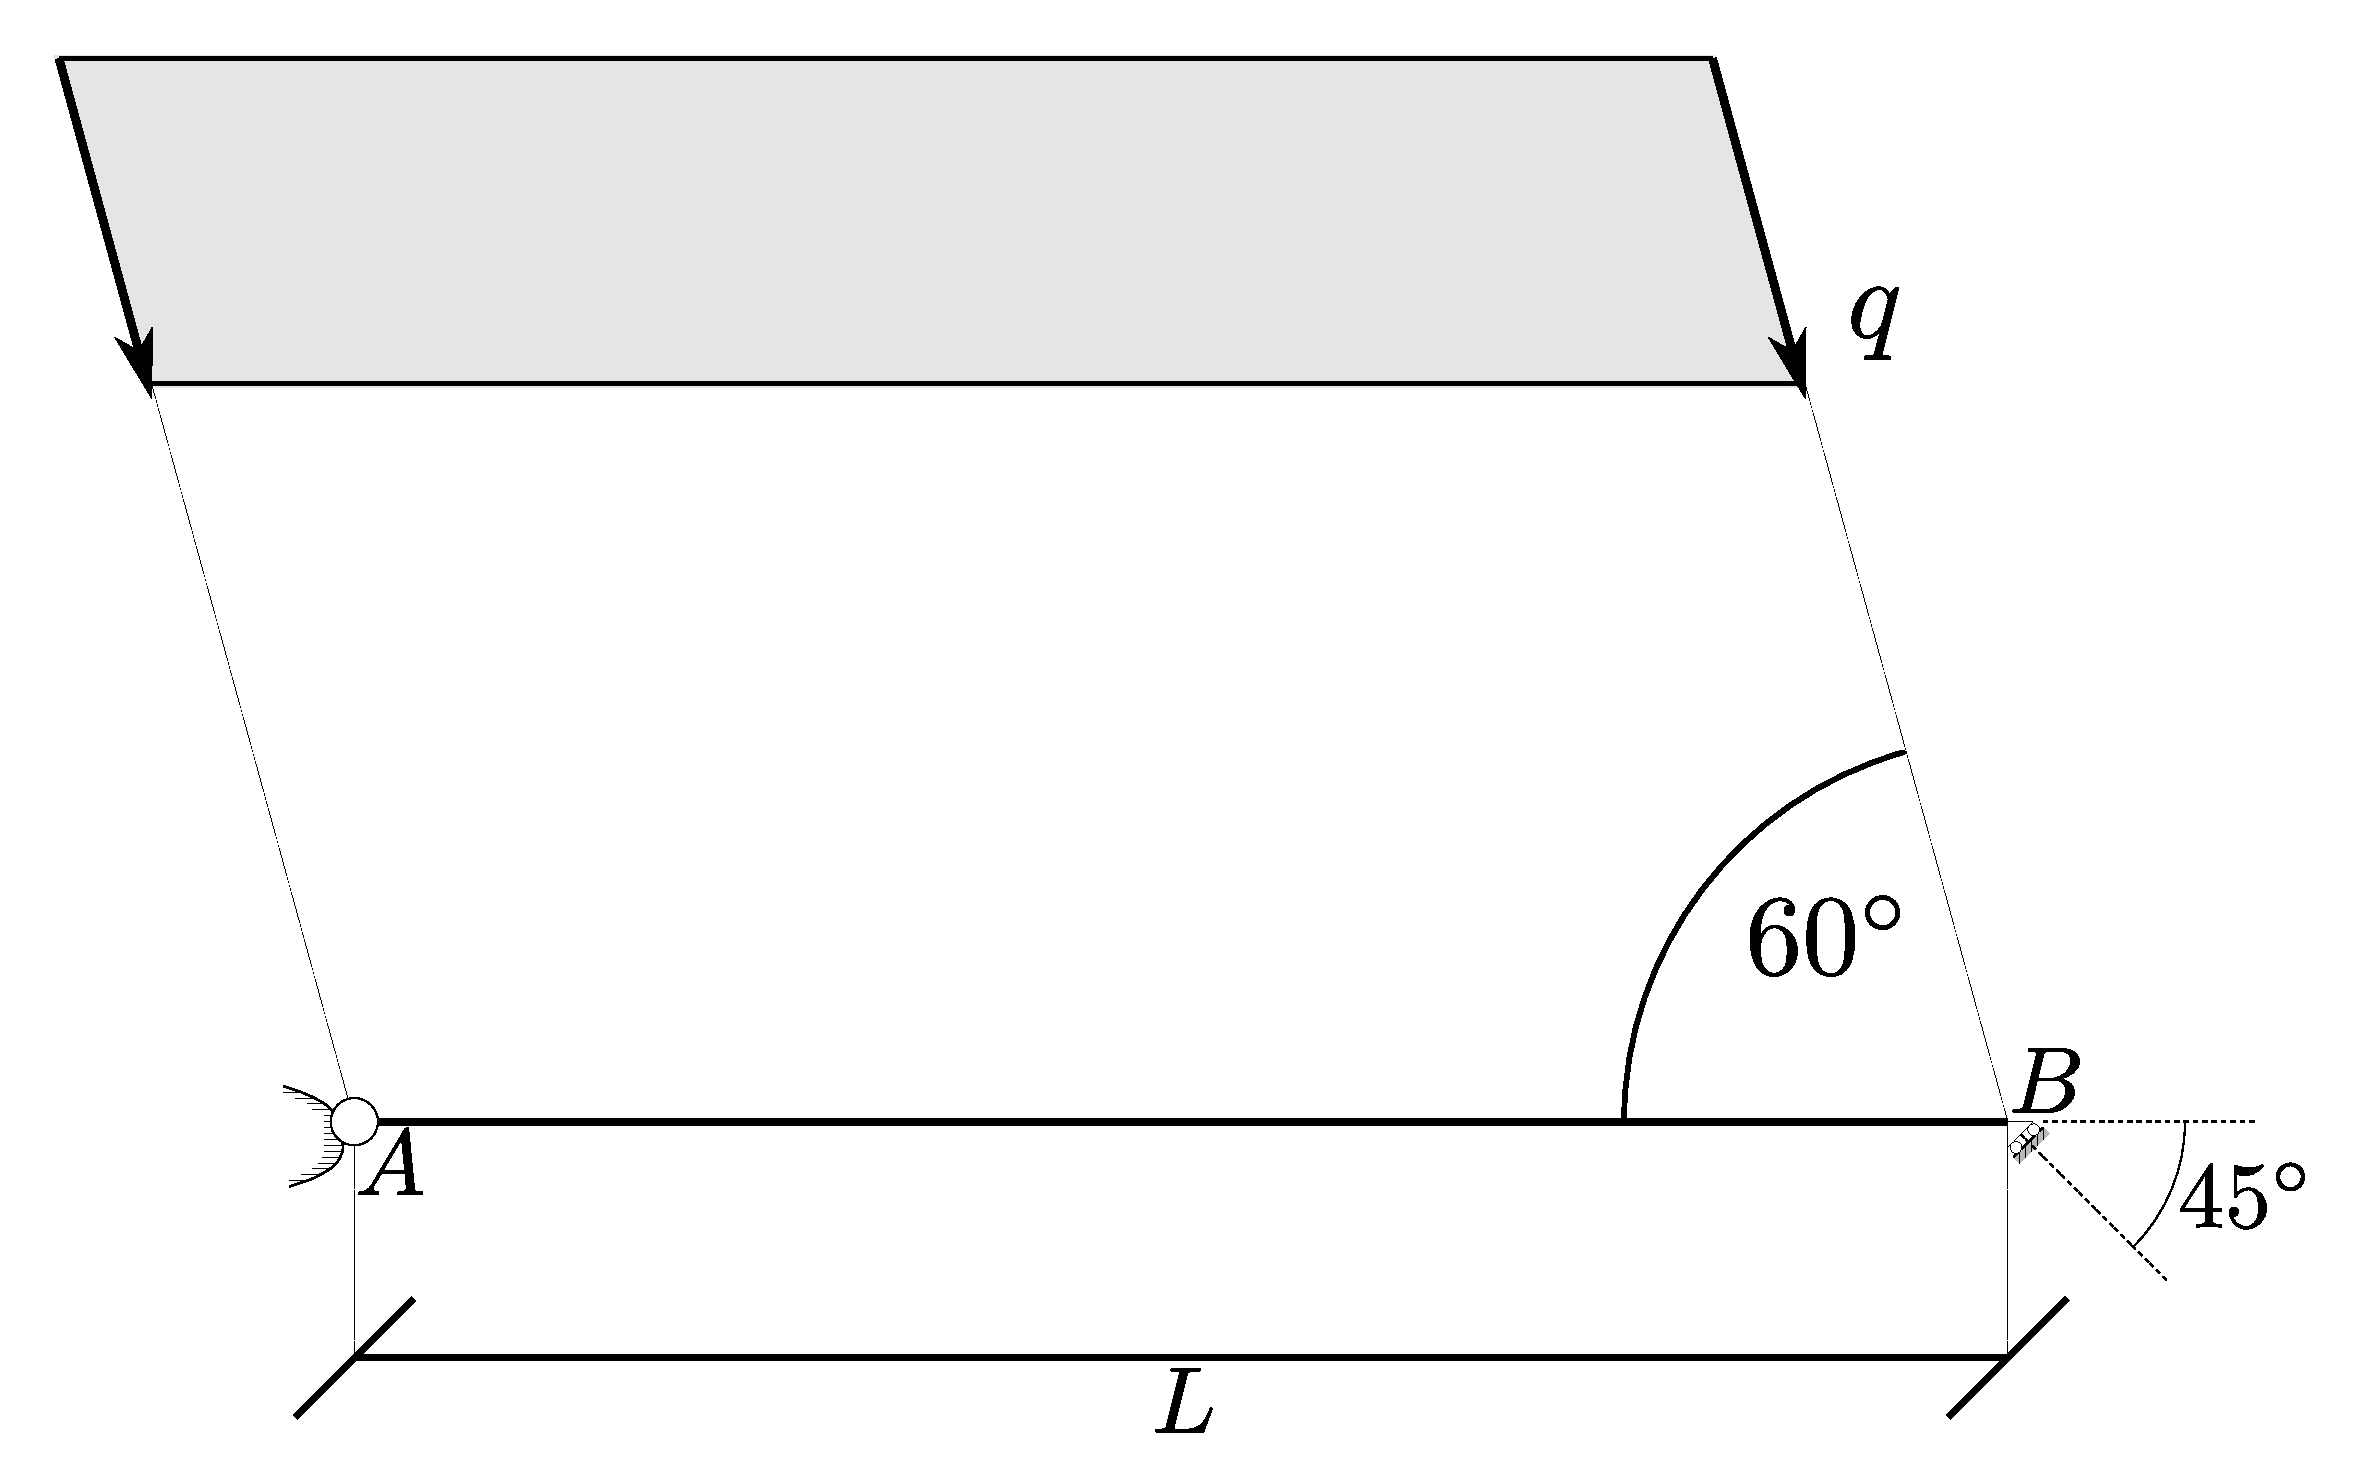
\includegraphics[width=0.65\textwidth]{Immagini/Parte_12/Esercizio12_1_1/esercizio12_1_1.pdf}
\caption{}
\label{Esercizio12-1-1}
\end{figure}
%--------------------------------------------------------------------------------------------------------------------------------------------------------------
Si chiede 
%----------------------------------------------------------------------------------------
\begin{enumerate}
\item di determinare le reazioni vincolari;
\item di scrivere le leggi di variazione delle funzioni $N=N(x)$, $T=T(x)$ ed $M=M(x)$ e tracciarne i diagrammi.
\end{enumerate}
%----------------------------------------------------------------------------------------
\subparagraph{Quesito 1}
%----------------------------------------------------------------------------------------
Si comincia imponendo l'equilibrio esterno, come si vede in figura~\ref{Esercizio12-1-2}:
%--------------------------------------------------------------------------------------------------------------------------------------------------------------
\renewcommand{\thefigure}{12.1~-~2}
\begin{figure}[ht]
\centering
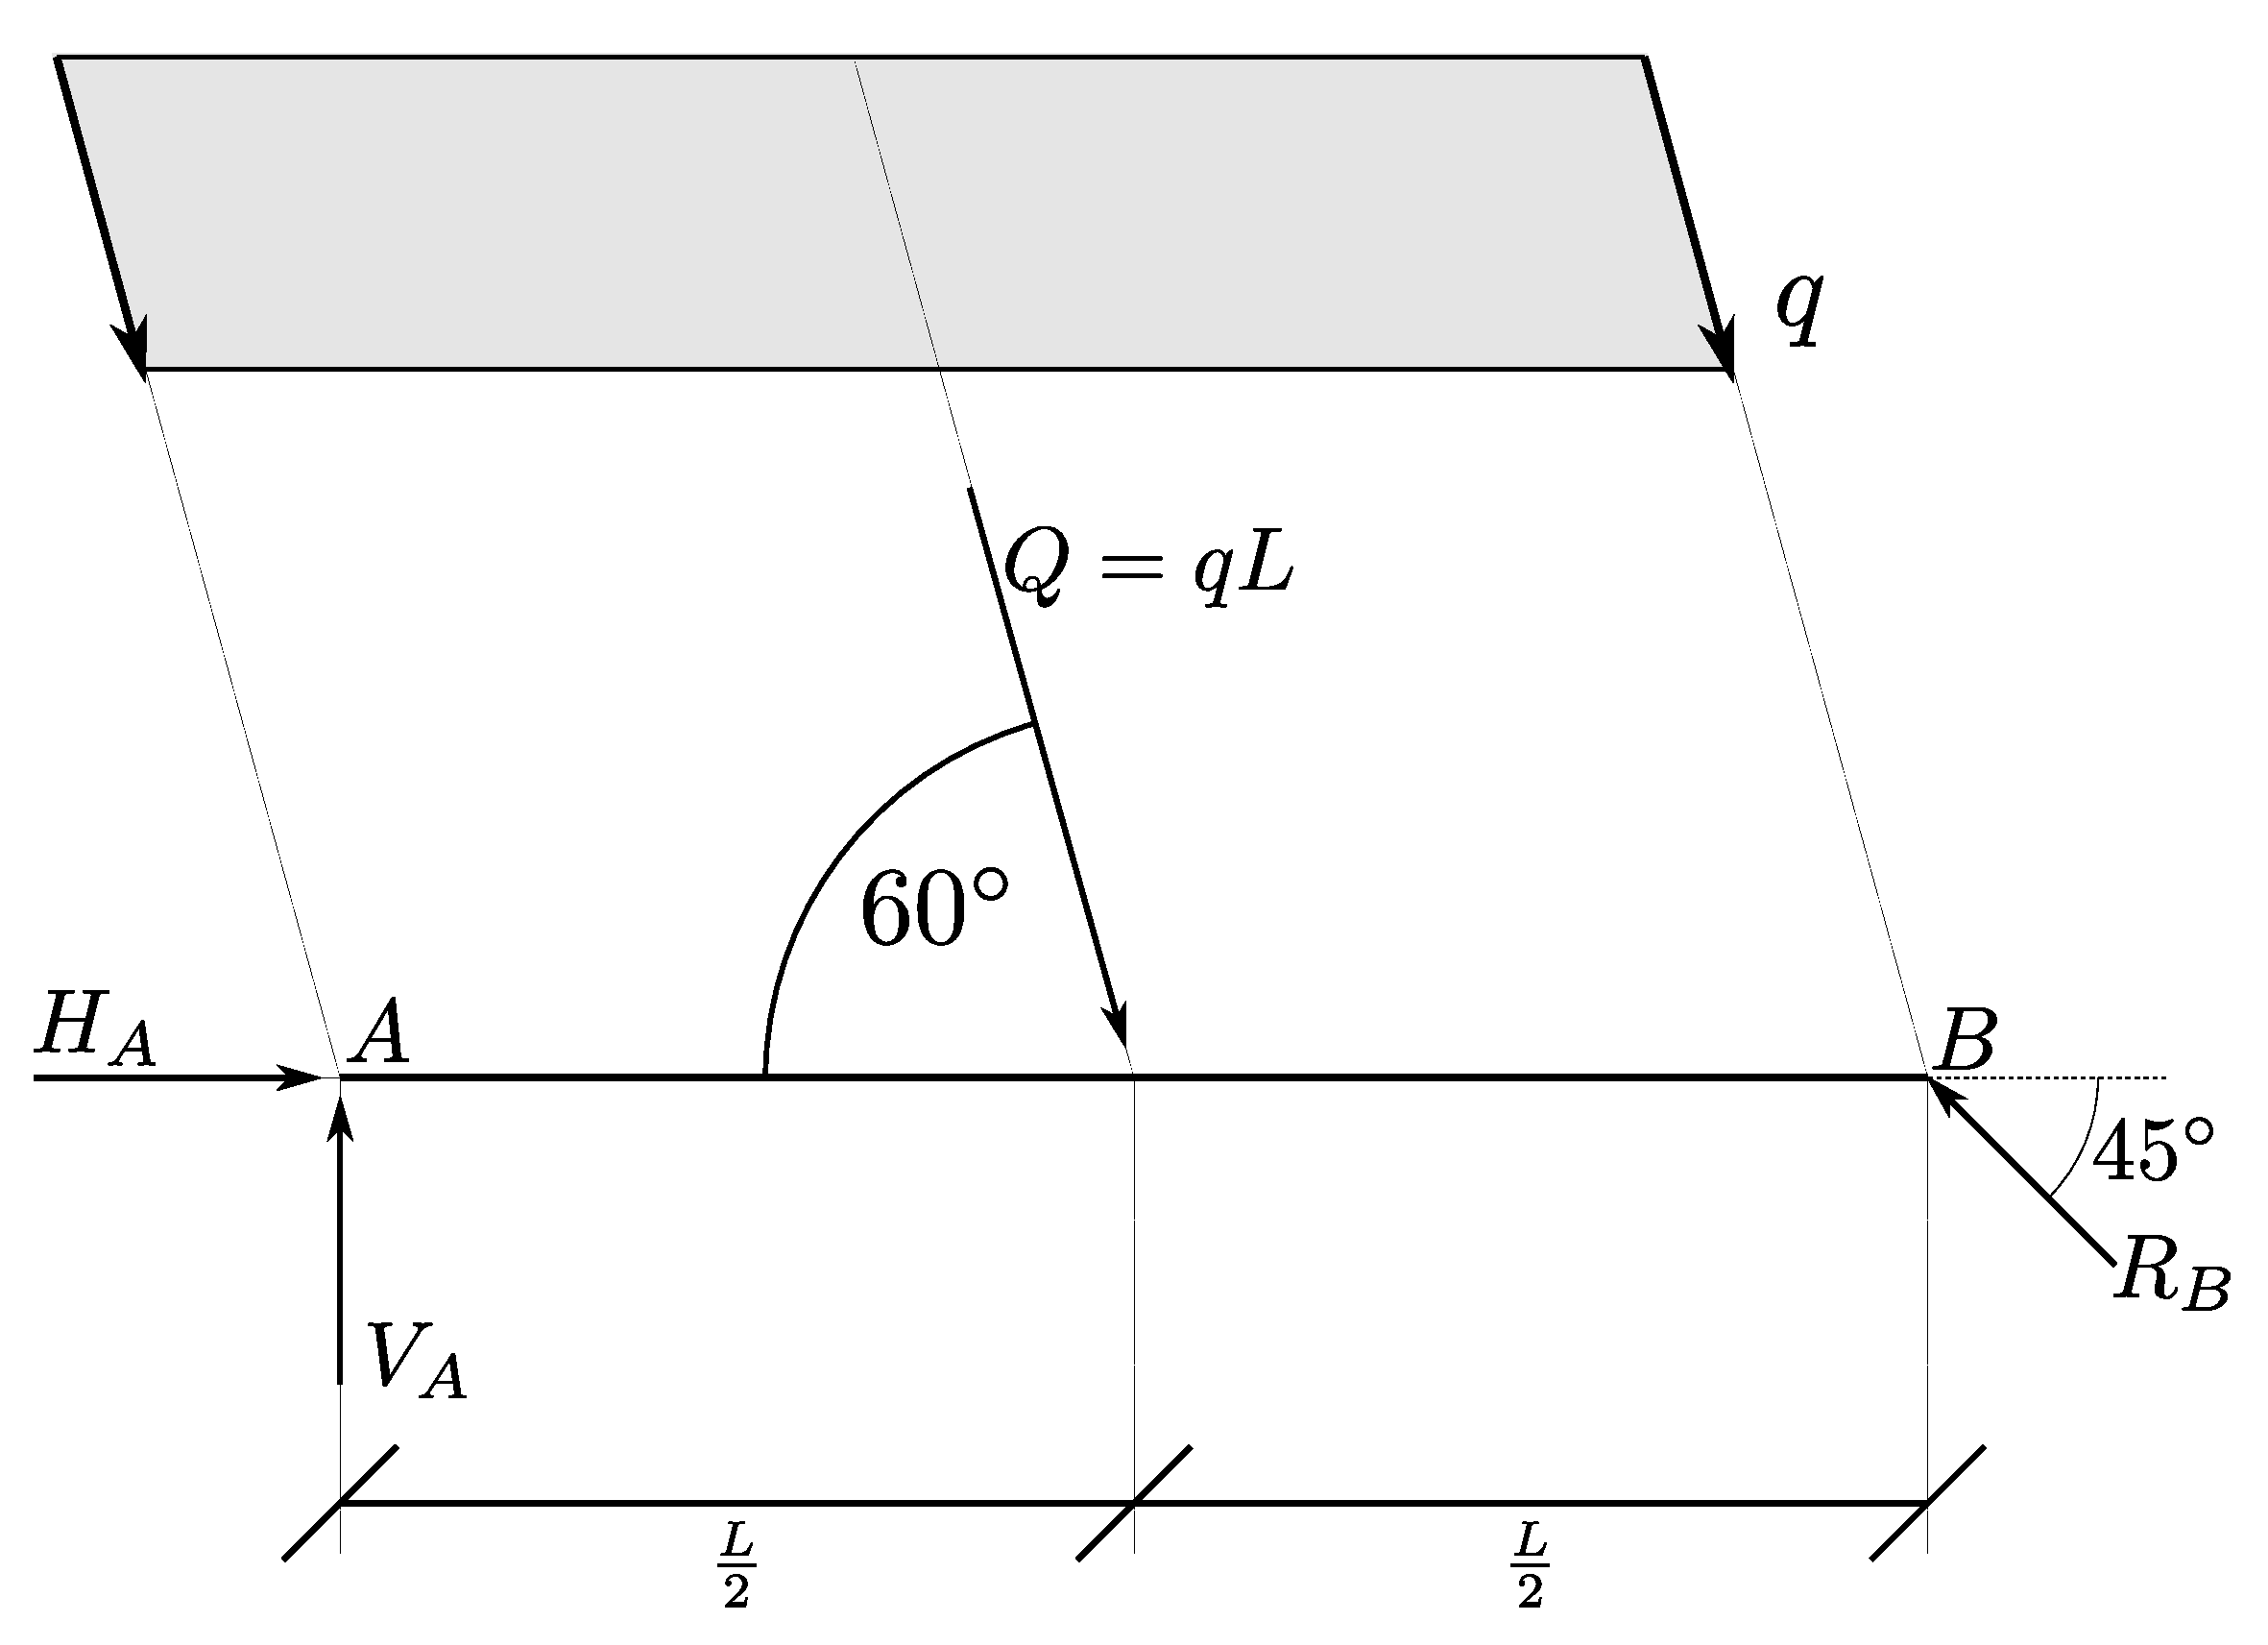
\includegraphics[width=0.65\textwidth]{Immagini/Parte_12/Esercizio12_1_1/esercizio12_1_2.pdf}
\caption{}
\label{Esercizio12-1-2}
\end{figure}
%--------------------------------------------------------------------------------------------------------------------------------------------------------------
\begin{align*}
-H_{A} + qL\cdot\cos{60^{\circ}} - \frac{\sqrt{2}}{2}R_{B} &= 0 \quad [\rightarrow] \\ 
V_{A} - qL\cdot \sin{60^{\circ}} + \frac{\sqrt{2}}{2}R_{B} &= 0 \quad [\uparrow] \\
-V_{A}\cdot L + qL\cdot \sin{60^{\circ}} \cdot \frac{L}{2} &= 0 \quad [B\,\circlearrowleft]
\end{align*}
%----------------------------------------------------------------------------------------
quindi
%--------------------------------------------------------------------------------------------------------------------------------------------------------------
\begin{align*}
H_{A} &= \frac{1}{2}\cdot qL - \frac{\sqrt{2}}{2}\cdot R_{B} = \frac{1}{2}\cdot qL - \frac{\sqrt{3}}{4}\cdot qL = \frac{2 - \sqrt{3}}{4}\cdot qL \quad [\leftarrow] \\ 
V_{A} &= \frac{1}{2}\cdot qL\cdot \sin{60^{\circ}} = \frac{\sqrt{3}}{4}\cdot qL  \quad [\uparrow] \\
R_{B} &= \sqrt{2}\biggl( qL\cdot \frac{\sqrt{3}}{2} - V_{A} \biggr) = \sqrt{2}\biggl(  \frac{\sqrt{3}}{2}\cdot qL - \frac{\sqrt{3}}{4}\cdot qL \biggr) = \frac{\sqrt{6}}{4}\cdot qL  \quad [\nwarrow]
\end{align*}
%----------------------------------------------------------------------------------------
ed in definitiva
%----------------------------------------------------------------------------------------
\begin{subequations}
\begin{align}
H_{A} &= \frac{2 - \sqrt{3}}{4}\cdot qL \quad [\leftarrow] \label{equazione12-1-1a} \tag{12.1.1a} \\
R_{B} &= \frac{\sqrt{6}}{4}\cdot qL  \quad [\nwarrow] \label{equazione12-1-1b} \tag{12.1.1b} \\ 
V_{A} &= \frac{\sqrt{3}}{4}\cdot qL \quad [\uparrow] \label{equazione12-1-1c} \tag{12.1.1c}
\end{align}
\end{subequations}
%----------------------------------------------------------------------------------------
\subparagraph{Quesito 2}
%----------------------------------------------------------------------------------------
%--------------------------------------------------------------------------------------------------------------------------------------------------------------
\renewcommand{\thefigure}{12.1~-~3}
\begin{figure}[ht]
\centering
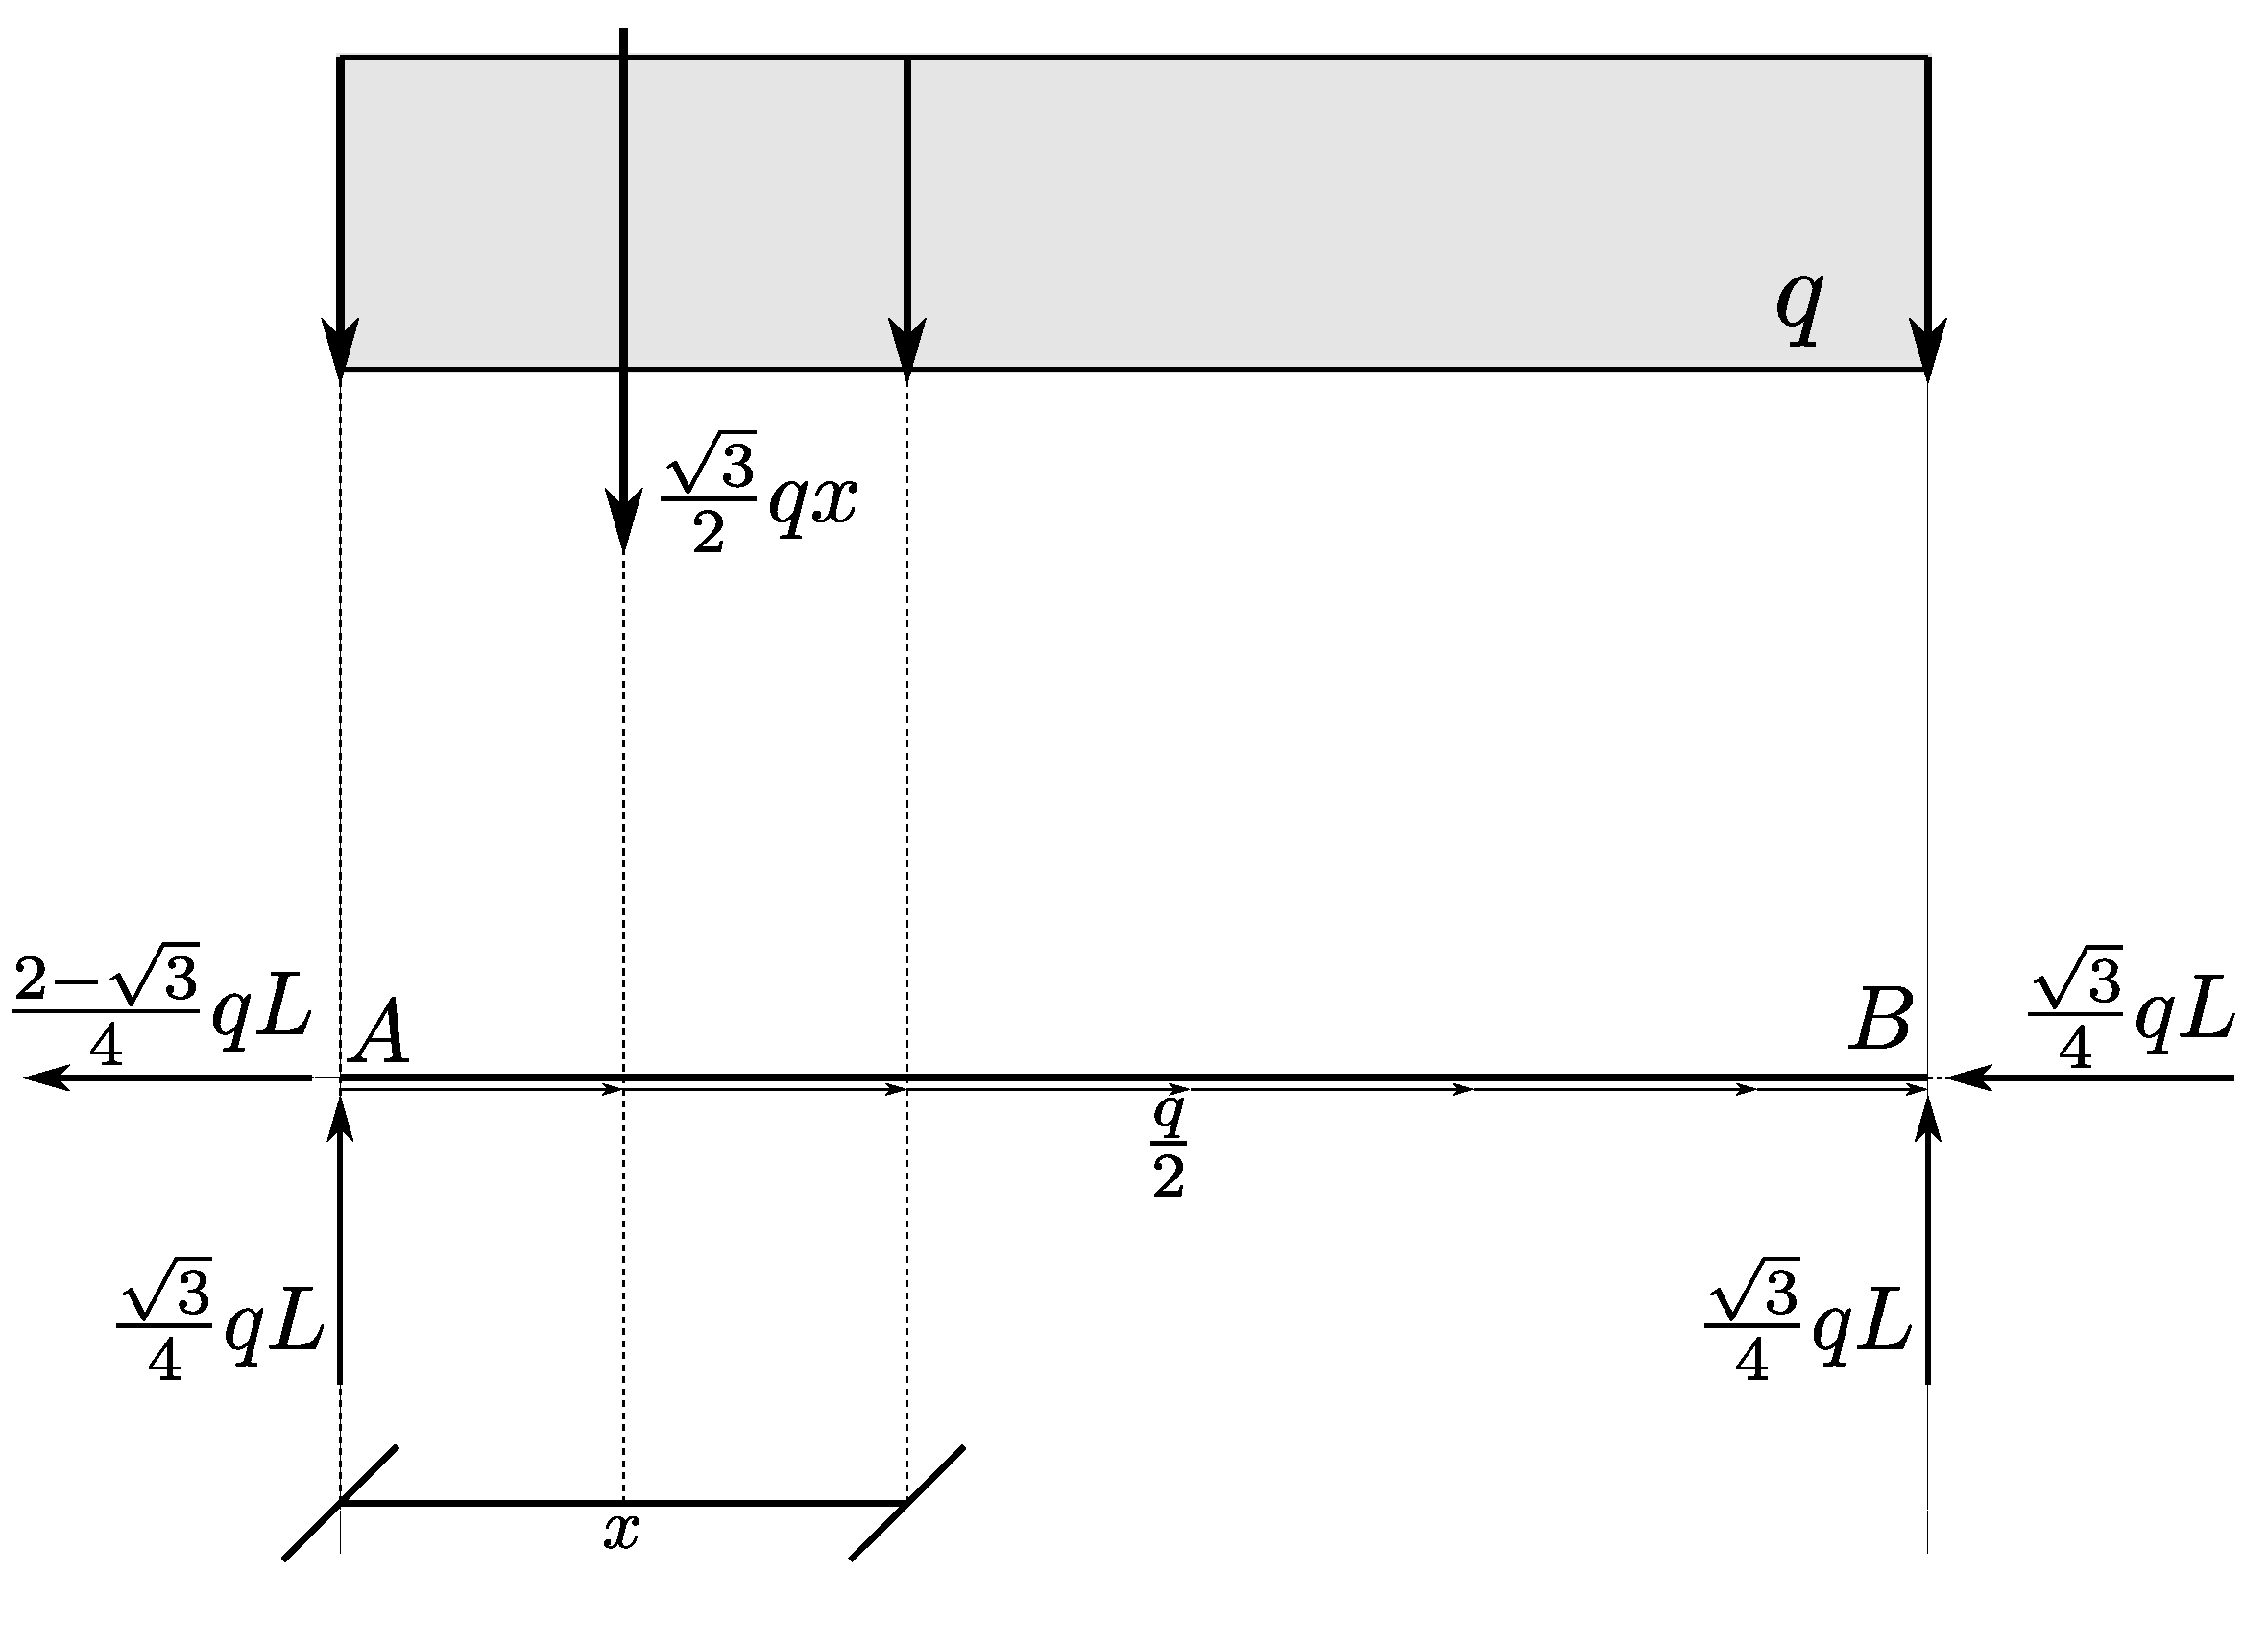
\includegraphics[width=0.65\textwidth]{Immagini/Parte_12/Esercizio12_1_1/esercizio12_1_3.pdf}
\caption{}
\label{Esercizio12-1-3}
\end{figure}
%--------------------------------------------------------------------------------------------------------------------------------------------------------------
%--------------------------------------------------------------------------------------------------------------------------------------------------------------
\renewcommand{\thefigure}{12.1~-~4}
\begin{figure}[ht]
\centering
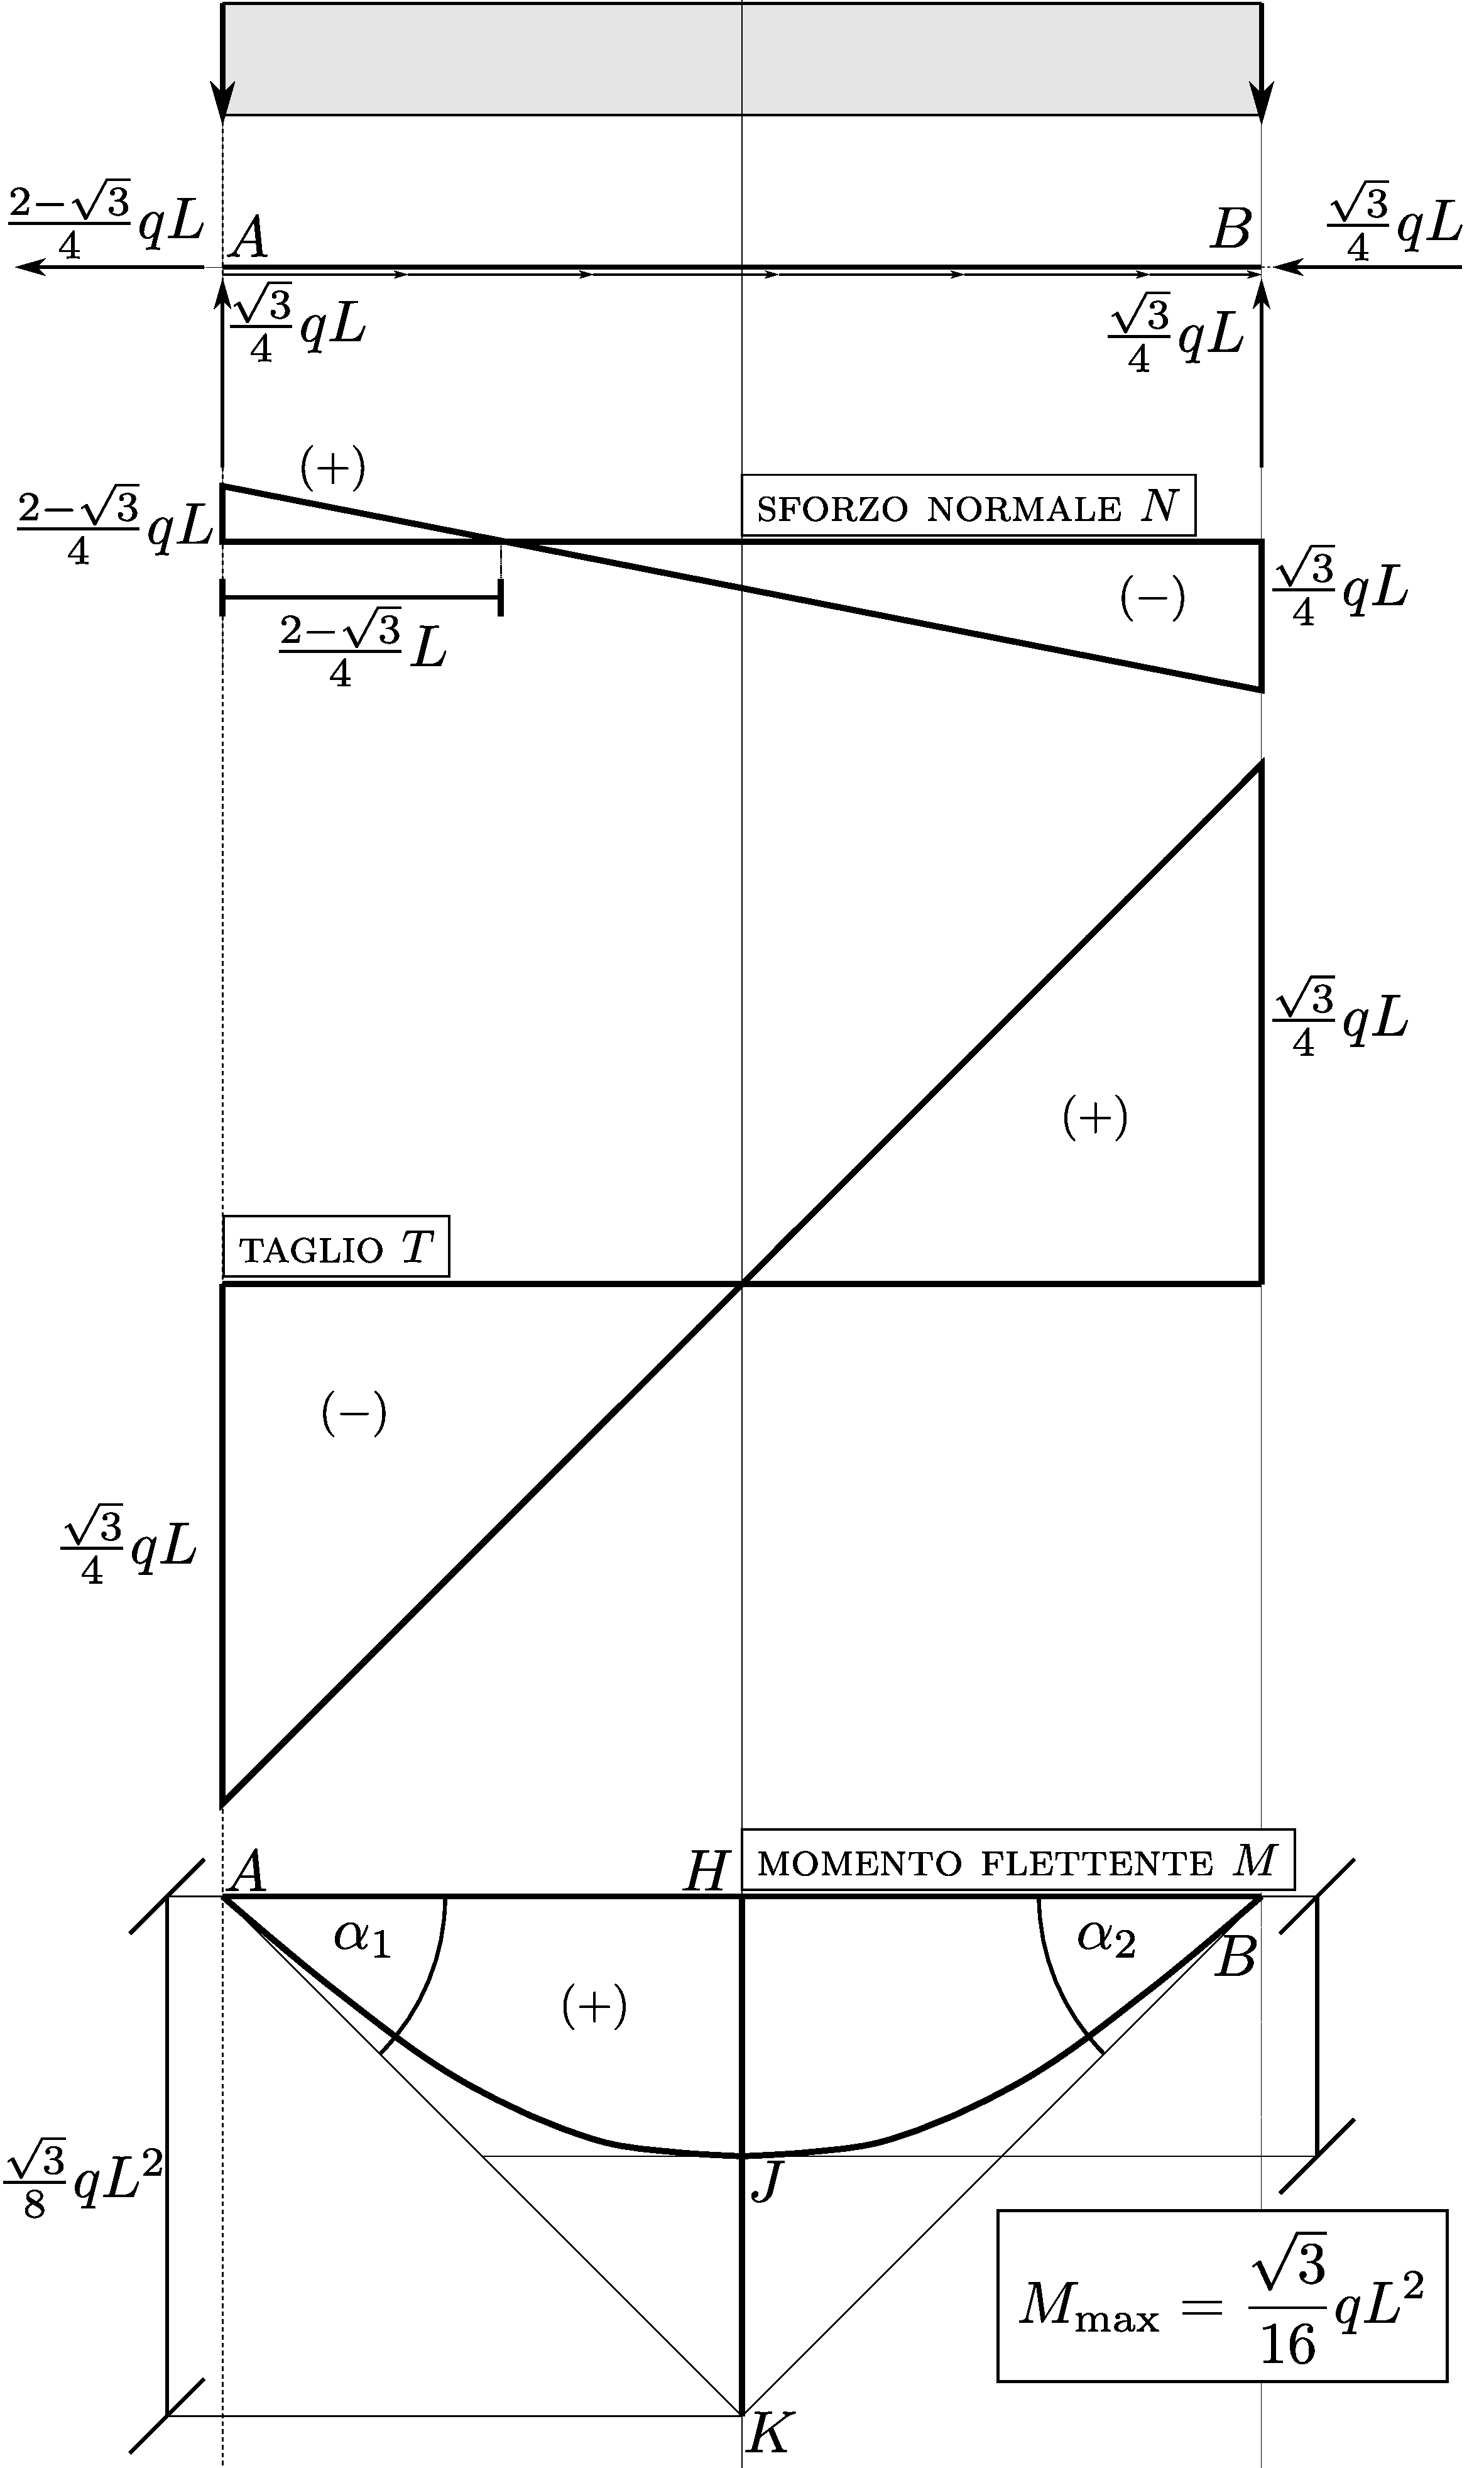
\includegraphics[width=0.8\textwidth]{Immagini/Parte_12/Esercizio12_1_1/esercizio12_1_4.pdf}
\caption{}
\label{Esercizio12-1-4}
\end{figure}
%--------------------------------------------------------------------------------------------------------------------------------------------------------------
Risulta conveniente scomporre il carico $q$ nelle direzioni assiale e trasversale
%----------------------------------------------------------------------------------------
\begin{equation*}
q = 
\begin{cases}
q_{x} &= \frac{1}{2}\cdot q            \notag \\
q_{y} &= -\frac{\sqrt{3}}{2}\cdot q  \notag 
\end{cases}
\end{equation*}
%----------------------------------------------------------------------------------------
Consideriamo la generica sezione $\mathcal{S}$ di ascissa $x$ come rappresentato in figura~\ref{Esercizio12-1-3} ed esplicitiamo $N$, $T$ ed $M$ applicando le definizioni:
%----------------------------------------------------------------------------------------
\begin{subequations}
\begin{align}
N(x) &= \frac{2 - \sqrt{3}}{4}\cdot qL - \frac{1}{2}\cdot qx = \frac{q}{4} \biggl[ (2 - \sqrt{3}) L - 2x \biggr]  \label{equazione12-1-2a} \tag{12.1.2a} \\
T(x) &= -\frac{\sqrt{3}}{4}\cdot qL + \frac{\sqrt{3}}{2}\cdot qx = \frac{\sqrt{3}}{4} q  (2x - L)  \label{equazione12-1-2b} \tag{12.1.2b} \\ 
M(x) &= \frac{\sqrt{3}}{4}\cdot qLx - \frac{\sqrt{3}}{2}\cdot qx \cdot \frac{x}{2} = \frac{\sqrt{3}}{4} q  (Lx - x^{2})  \label{equazione12-1-2c} \tag{12.1.2c}
\end{align}
\end{subequations}
%----------------------------------------------------------------------------------------
Come preannunciato dalle proposizioni enunciate in precedenza, $N(x)$ e $T(x)$ sono \textsc{funzioni lineari} ed $M(x)$ è \textsc{funzione quadratica}. I diagrammi di $N$ e $T$, essendo lineari, si tracceranno facilmente una volta calcolati i valori agli estremi. Il diagramma di $M$ sarà invece una \textsc{parabola} e, pertanto, merita alcune precisazioni; osserviamo, intanto, che dalla legge di variazione di $M$ si trae immediatamente che $M=0$ per $x=0$ e per $x=L$. Risulta altrettanto facile verificare che 
%----------------------------------------------------------------------------------------
\begin{equation*}
\boxed{ M\biggl( x=\frac{L}{2} \biggr) = \frac{\sqrt{3}}{16} qL^{2} }
\end{equation*}
%----------------------------------------------------------------------------------------
In mezzeria, deve risultare inoltre 
%----------------------------------------------------------------------------------------
\begin{equation*}
\boxed{ \frac{dM}{dx} = T\biggl(  x=\frac{L}{2} \biggr) = 0 }
\end{equation*}
%----------------------------------------------------------------------------------------
e quindi resta dimostrato che in mezzeria \textbf{il momento flettente} $\mathbf{M}$ \textbf{ha un massimo relativo}, che in questo caso particolare è anche massimo assoluto. Per disegnare in maniera \emph{decente} la parabola è, tuttavia, opportuno tracciare almeno le rette tangenti agli estremi; a tal fine, si procede così:
%----------------------------------------------------------------------------------------
\begin{enumerate}
\item il coefficiente della retta tangente alla parabola nell'estremo sinistro è, ovviamente, in valore assoluto 
\begin{equation*}
\boxed{ \abs{\tan{\alpha_{1}}} = \abs*{\frac{dM}{dx}}_{x=0} = T_{A} = \frac{\sqrt{3}}{4}qL }
\end{equation*}
\item si calcola il valore che la tangente $A_{1}$ calcolata raggiunge in mezzeria
\begin{equation*}
\boxed{ \abs{HK} = \frac{L}{2} \abs{\tan{\alpha_{1}}} = T_{A} = \frac{\sqrt{3}}{8}qL^{2} }
\end{equation*}
che corrisponde a due volte il valore del momento flettente calcolato in $x=\frac{L}{2}$; 
\item è noto che la parabola gode della seguente proprietà: 
\begin{propr}
Considerate le due rette tangenti in due punti qualsiasi di una parabola, esse si intersecano in corrispondenza del punto posto alla metà della distanza tra i suddetti punti.
\end{propr}
In pratica, le due rette tangenti si intersecano \emph{a metà strada}; e così si può disegnare automaticamente la tangente all'estremo destro, senza la necessità di svolgere conti analoghi a quelli già effettuati;
\item osserviamo, infine, che a proposito del diagramma del momento flettente $M$, è molto diffusa la convenzione di disegnare il diagramma \textbf{\textsc{dalla parte delle fibre tese}} e cioè
\begin{equation*}
\boxed{
M>0 \,\, \longrightarrow \,\, M \text{ tende le fibre inferiori} \,\, \longrightarrow \,\, \text{Ordinata positiva di } M \text{ sotto}
}
\end{equation*}
\end{enumerate}
%----------------------------------------------------------------------------------------
Risulta pertanto possibile tracciare il diagramma del momento flettente seguendo questa procedura, del tutto generale. I diagrammi di $N(x)$, $T(x)$ ed $M(x)$ vengono riportati in figura~\ref{Esercizio12-1-4}.
%--------------------------------------------------------------------------------------------------------------------------------------------------------------
\clearpage
\paragraph{Esercizio 12.2}
%--------------------------------------------------------------------------------------------------------------------------------------------------------------
\renewcommand{\thefigure}{12.2~-~1}
\begin{figure}[ht]
\centering
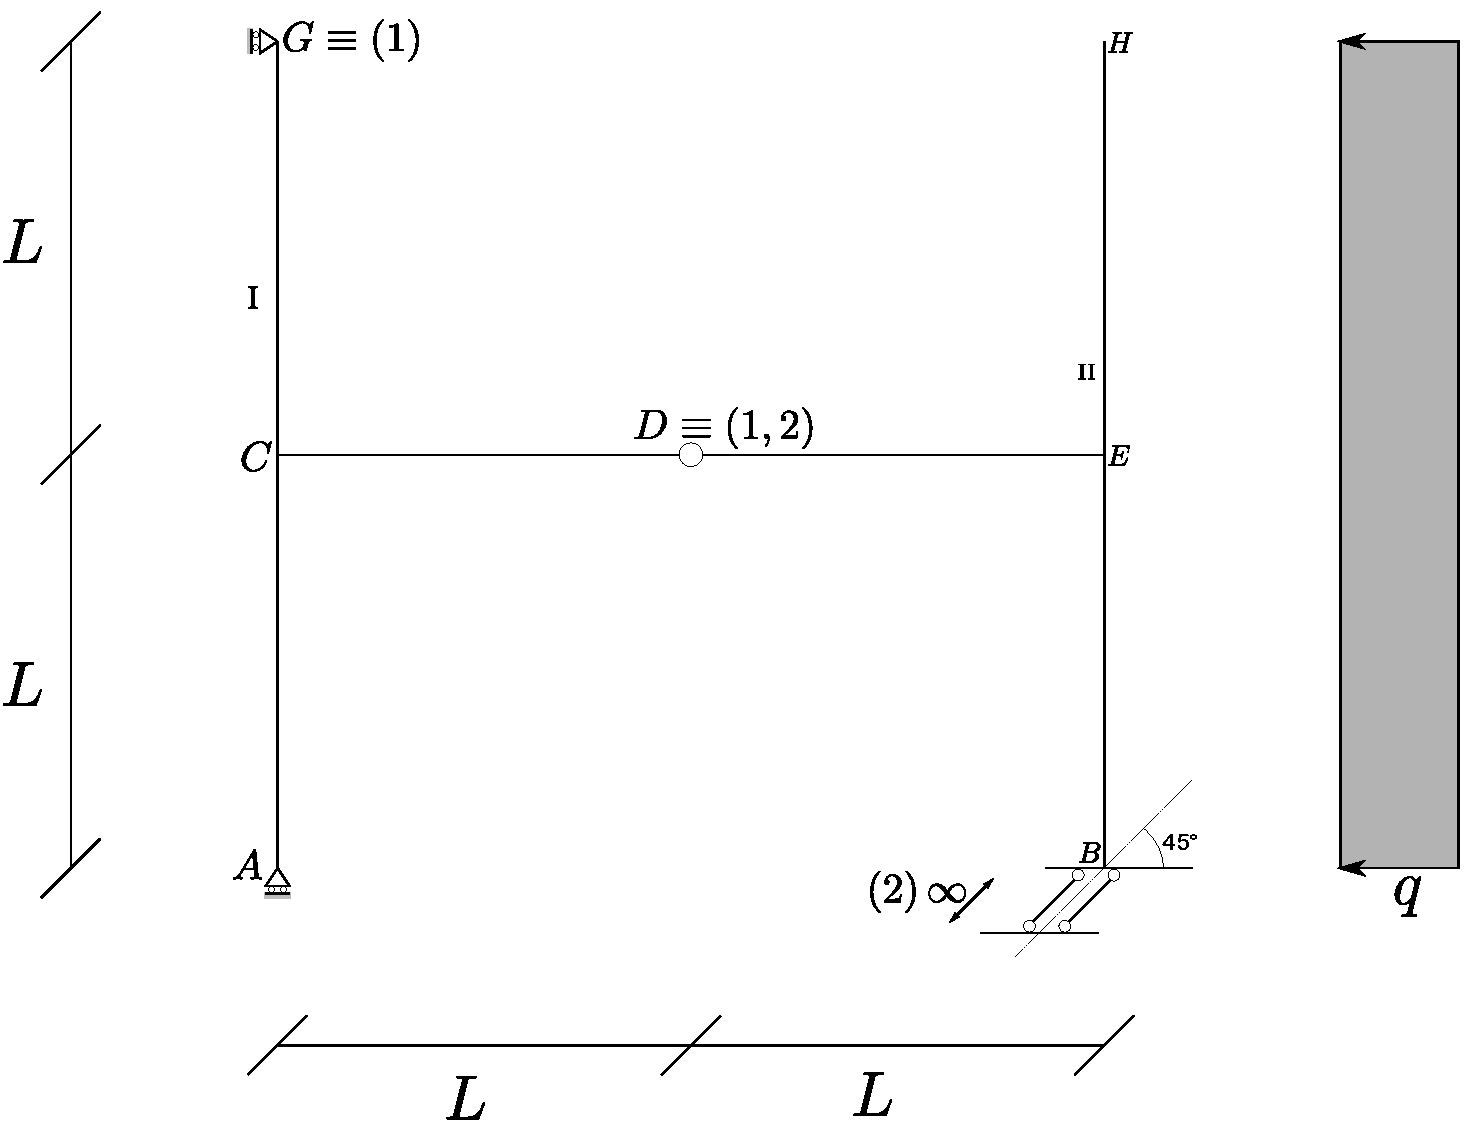
\includegraphics[width=\textwidth]{Immagini/Parte_12/Esercizio12_2/12_2_1.pdf}
\caption{}
\label{Esercizio12-2-1}
\end{figure}
%--------------------------------------------------------------------------------------------------------------------------------------------------------------
Si chiede 
%----------------------------------------------------------------------------------------
\begin{enumerate}
\item di classificare la struttura;
\item di determinare le reazioni vincolari;
\item di tracciare i diagrammi di $N$, $T$ ed $M$.
\end{enumerate}
%----------------------------------------------------------------------------------------
\subparagraph{Quesito 1}
%----------------------------------------------------------------------------------------
Abbiamo una struttura composta da due tronchi. Risulta:
%----------------------------------------------------------------------------------------
\begin{align*}
m &= 3\times 2 = 6 \\ 
n &= 1A + 2B + 2D + 1G = 6
\end{align*}
%----------------------------------------------------------------------------------------
Pertanto, $m - n = l - i = 0$; i centri $(1)$, $(1, 2)$ e $(2)$ sono univocamente determinati e non sono allineati. Risulta, allora che $l=0$; anche $i$ sarà nulla e, dunque, la struttura è \textsc{isostatica}.
%----------------------------------------------------------------------------------------
\subparagraph{Quesito 2}
%----------------------------------------------------------------------------------------
Cominciamo a ragionare sull'equilibrio del primo tronco, che è una volta iperstatico ed è esente da carichi attivi. Su di esso agiscono tre forze: $R_{A}$, $R_{G}$ ed $R_{D}$. Esse devono concorrere in un punto e per questo $R_D$ passerà necessariamente per il punto $G$. Essendo nota la retta d'azione di $R_{D}$, il secondo tronco è \textbf{diventato staticamente determinato} e, pertanto, siamo in grado di scriverne le equazioni di equilibrio. Si ha:
%----------------------------------------------------------------------------------------
\begin{align*}
\frac{\sqrt{2}}{2} R_{D} + \frac{\sqrt{2}}{2} R_{B} - 2qL &= 0 \quad [\leftarrow] \\ 
\frac{\sqrt{2}}{2} R_{B} - \frac{\sqrt{2}}{2} R_{D}          &= 0 \quad [\uparrow] \\
\mathcal{M}_{B} + 2qL^{3}                                          &= 0 \quad [B\, \circlearrowleft] 
\end{align*}
%----------------------------------------------------------------------------------------
Risolvendo il sistema si trova
%----------------------------------------------------------------------------------------
\begin{subequations}
\begin{align}
R_{B}                &= \sqrt{2}qL  \quad [\nearrow] \label{equazione12-2-1a} \tag{12.2.1a} \\
R_{D}                &= \sqrt{2}qL  \quad [\searrow] \label{equazione12-2-1b} \tag{12.2.1b} \\ 
\mathcal{M}_{B} &= -2qL^{3} \quad [\circlearrowright] \label{equazione12-2-1c} \tag{12.2.1c}
\end{align}
\end{subequations}
%----------------------------------------------------------------------------------------
Adesso possiamo rapidamente determinare $R_{A}$ ed $R_{G}$ imponendo l'equilibrio del primo tronco; a tal proposito, osserviamo che $R_{A}$ ed $R_{G}$ si potranno determinare imponendo che il poligono da esse formato con $R_{D} [\swarrow]$ sia chiuso. Quindi 
%----------------------------------------------------------------------------------------
\begin{equation*}
\text{Reazioni } R_{A} \text{ ed } R_{G}
\begin{cases}
R_{A} &=  qL           \notag \\
R_{G} &= qL  \notag 
\end{cases}
\end{equation*}
%----------------------------------------------------------------------------------------
Si riporta il quadro completo delle reazioni in figura. 
%--------------------------------------------------------------------------------------------------------------------------------------------------------------
\renewcommand{\thefigure}{12.2~-~2}
\begin{figure}[ht]
\centering
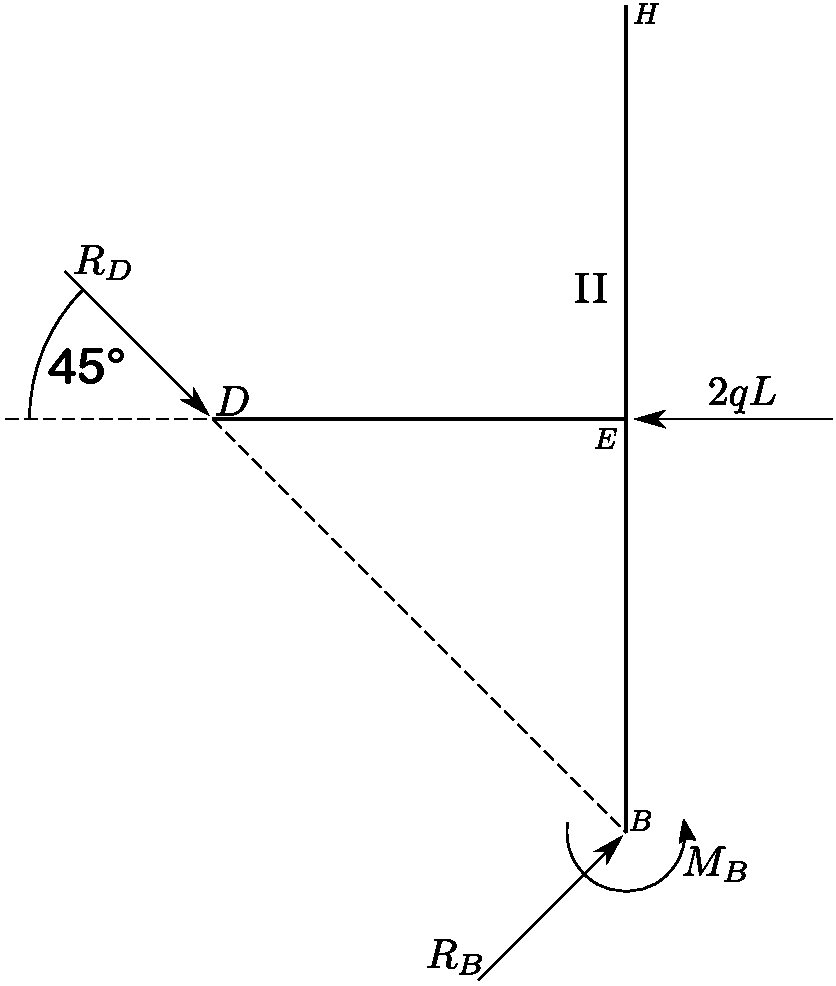
\includegraphics[width=0.55\textwidth]{Immagini/Parte_12/Esercizio12_2/12_2_2.pdf}
\caption{}
\label{Esercizio12-2-2}
\end{figure}
%--------------------------------------------------------------------------------------------------------------------------------------------------------------
%--------------------------------------------------------------------------------------------------------------------------------------------------------------
\renewcommand{\thefigure}{12.2~-~3}
\begin{figure}[ht]
\centering
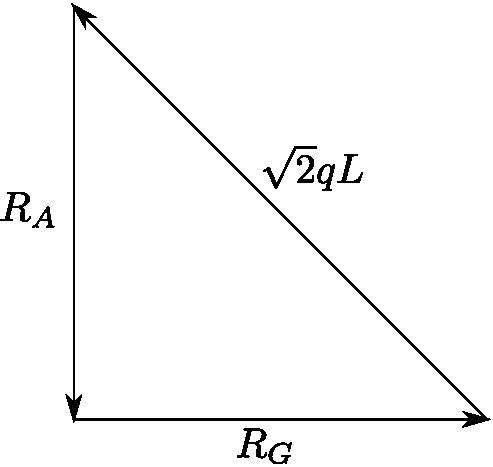
\includegraphics[width=0.35\textwidth]{Immagini/Parte_12/Esercizio12_2/12_2_3.pdf}
\caption{}
\label{Esercizio12-2-3}
\end{figure}
%--------------------------------------------------------------------------------------------------------------------------------------------------------------
%--------------------------------------------------------------------------------------------------------------------------------------------------------------
\renewcommand{\thefigure}{12.2~-~4}
\begin{figure}[ht]
\centering
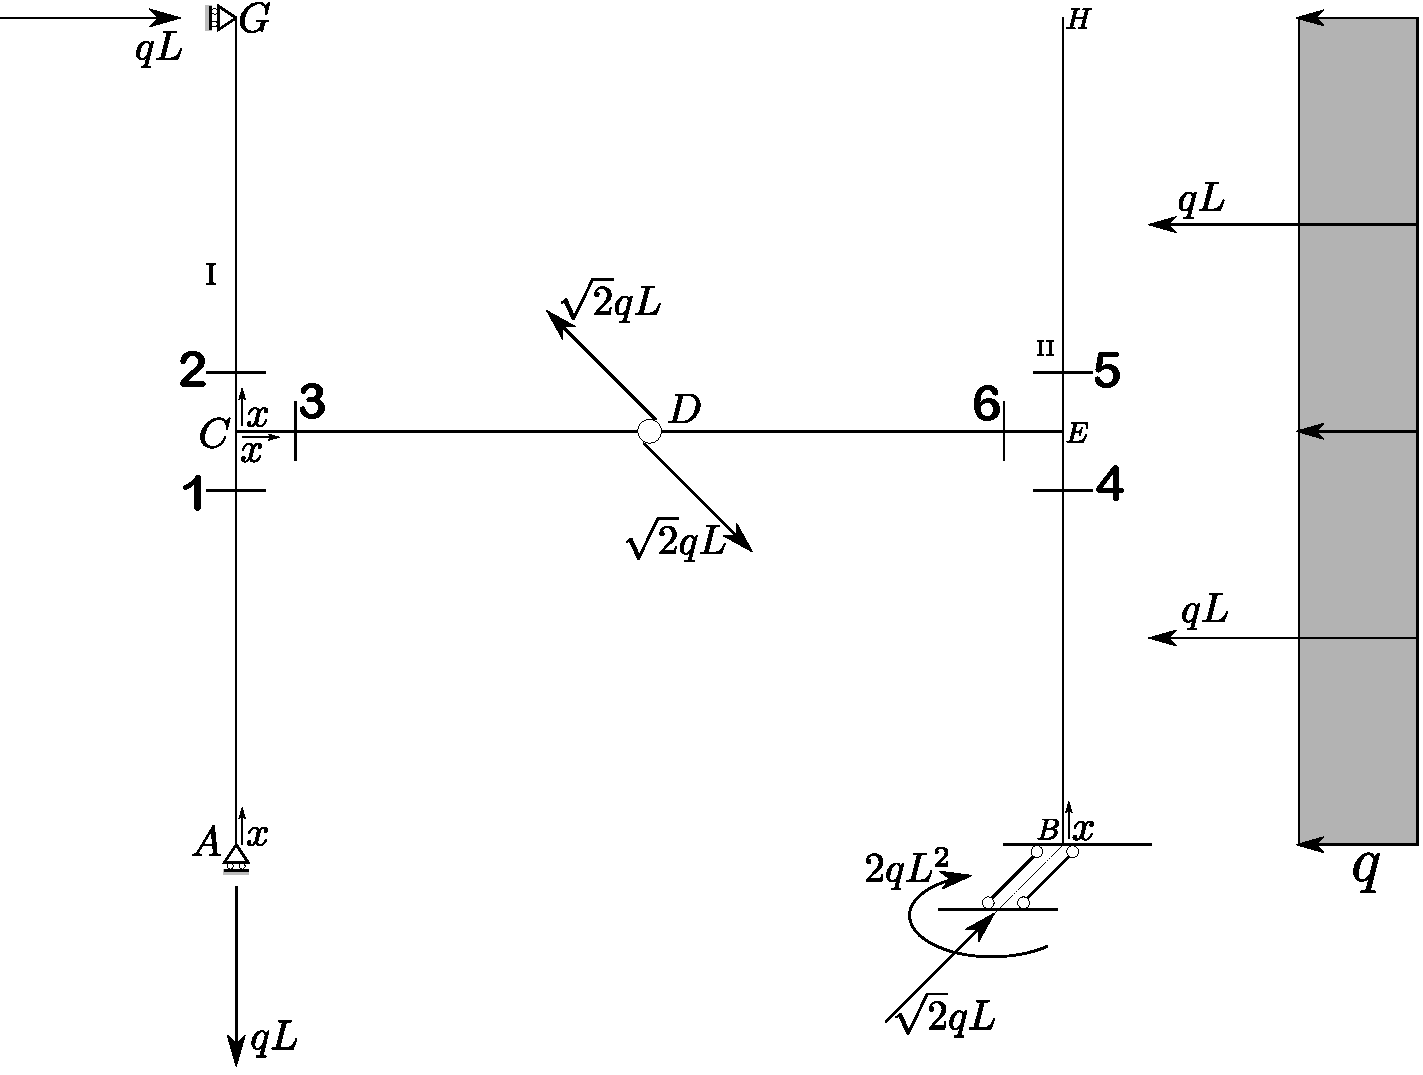
\includegraphics[width=\textwidth]{Immagini/Parte_12/Esercizio12_2/12_2_4.pdf}
\caption{}
\label{Esercizio12-2-4}
\end{figure}
%--------------------------------------------------------------------------------------------------------------------------------------------------------------
%--------------------------------------------------------------------------------------------------------------------------------------------------------------
\renewcommand{\thefigure}{12.2~-~5}
\begin{figure}[ht]
\centering
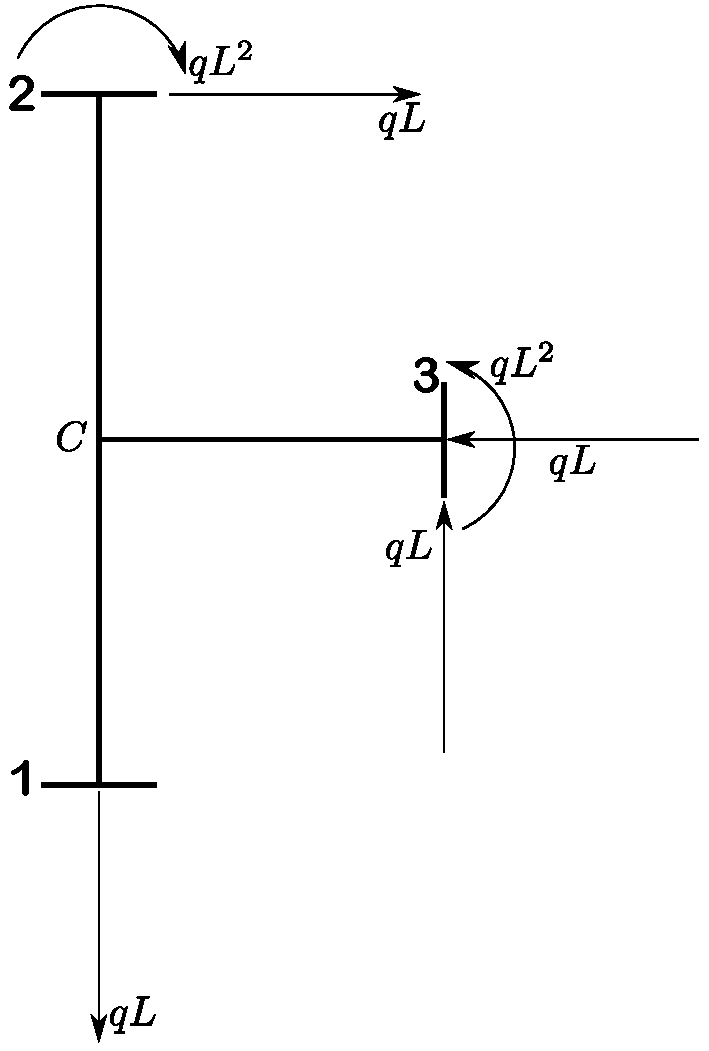
\includegraphics[width=0.45\textwidth]{Immagini/Parte_12/Esercizio12_2/12_2_5.pdf}
\caption{}
\label{Esercizio12-2-5}
\end{figure}
%--------------------------------------------------------------------------------------------------------------------------------------------------------------
%--------------------------------------------------------------------------------------------------------------------------------------------------------------
\renewcommand{\thefigure}{12.2~-~6}
\begin{figure}[ht]
\centering
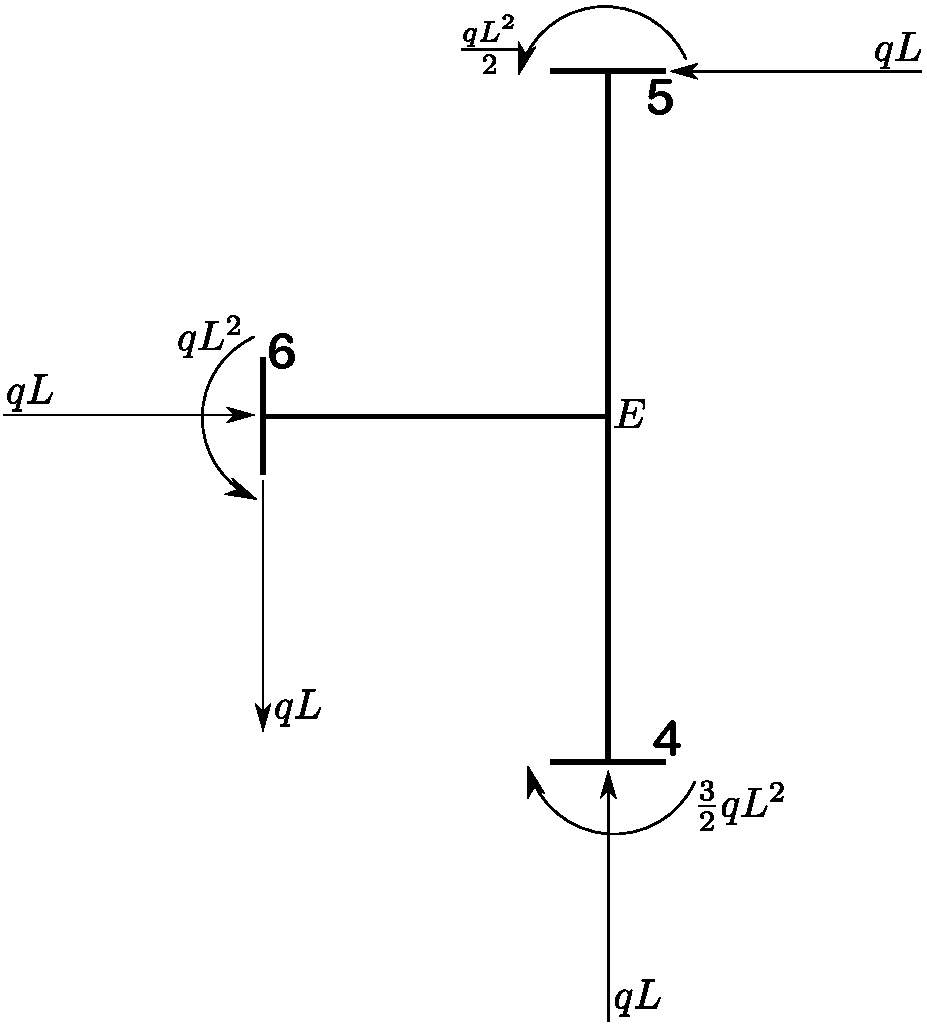
\includegraphics[width=0.45\textwidth]{Immagini/Parte_12/Esercizio12_2/12_2_6.pdf}
\caption{}
\label{Esercizio12-2-6}
\end{figure}
%--------------------------------------------------------------------------------------------------------------------------------------------------------------
%----------------------------------------------------------------------------------------
\subparagraph{Quesito 3}
%----------------------------------------------------------------------------------------
Prima di tracciare i diagrammi della sollecitazione interna, è opportuno calcolare i valori di $N$, $T$ ed $M$ agli estremi di ciascun tratto. A tale scopo, il carico è stato interrotto in $E$ e si sono segnate le risultanti dei tratti $BE$ ed $EH$. Ai fini di attribuire il giusto segno ad $M$, si sono assunti a piacere i versi degli assi $x$ sui vari tratti rettilinei della struttura. Si osservi attentamente la figura prima di procedere. E allora andiamo a fare i conti:
%----------------------------------------------------------------------------------------
\begin{equation*}
\text{Tratto } A-1
\begin{cases}
M_{A} &= 0; \quad T_{A} = 0; \quad  N_{A} = qL  \notag \\
M_{1} &= 0; \quad T_{1} = 0;  \quad N_{1} = qL  \notag 
\end{cases}
\end{equation*}
%----------------------------------------------------------------------------------------
%----------------------------------------------------------------------------------------
\begin{equation*}
\text{Tratto } B - 4
\begin{cases}
M_{B} &= 2qL^{2}; \quad T_{B} = qL; \quad  N_{B} = -qL  \notag \\
M_{4} &= 2qL^{2} - qL\cdot L + qL \cdot \frac{L}{2} = \frac{3}{2}\cdot qL^{2}; \quad T_{4} = qL - qL = 0;  \quad N_{4} = -qL  \notag 
\end{cases}
\end{equation*}
%----------------------------------------------------------------------------------------
%----------------------------------------------------------------------------------------
\begin{equation*}
\text{Tratto } 2-G
\begin{cases}
M_{2} &= -qL^{2}; \quad T_{2} = -qL; \quad  N_{2} = 0  \notag \\
M_{G} &= 0; \quad T_{G} = - qL;  \quad N_{G} = 0  \notag 
\end{cases}
\end{equation*}
%----------------------------------------------------------------------------------------
%----------------------------------------------------------------------------------------
\begin{equation*}
\text{Tratto } 5 - H
\begin{cases}
M_{5} &= \frac{qL^{2}}{2}; \quad T_{5} = qL; \quad  N_{5} = 0  \notag \\
M_{H} &= 0; \quad T_{H} = - qL;  \quad N_{H} = 0  \notag 
\end{cases}
\end{equation*}
%----------------------------------------------------------------------------------------
%----------------------------------------------------------------------------------------
\begin{equation*}
\text{Tratto } 3 - D_{s}
\begin{cases}
M_{3} &= qL^{2}; \quad T_{3} = qL; \quad  N_{3} = -qL  \notag \\
M_{\textup{D, s}} &= 0; \quad T_{\textup{D, s}} = qL;  \quad N_{\textup{D, s}} = -qL  \notag 
\end{cases}
\end{equation*}
%----------------------------------------------------------------------------------------
%----------------------------------------------------------------------------------------
\begin{equation*}
\text{Tratto } D_{d} - 6
\begin{cases}
M_{\textup{D, d}} &= 0; \quad T_{\textup{D, d}} = qL; \quad  N_{\textup{D, d}} = -qL  \notag \\
M_{6} &= -qL^{2}; \quad T_{6} = qL;  \quad N_{6} = -qL  \notag 
\end{cases}
\end{equation*}
%----------------------------------------------------------------------------------------
I valori di $N$, $T$ ed $M$ calcolati nelle sezioni $1$, $2$, $3$, $4$, $5$ e $6$ sono verificabili controllando gli equilibri di ciascun nodo triplo. Si ha:
%----------------------------------------------------------------------------------------
\begin{align*}
qL - qL              &= 0 \quad [\textsc{ok}] \\ 
-qL + qL            &= 0 \quad [\textsc{ok}] \\
qL^{2} - qL^{2} &= 0 \quad [\textsc{ok}] 
\end{align*}
%----------------------------------------------------------------------------------------
Si noti che i segmentini $C1$, $C2$ e $C3$ hanno lunghezza infinitesima; pertanto le forze avranno braccio pressocché nullo rispetto al punto $C$. 
%----------------------------------------------------------------------------------------
\begin{align*}
qL - qL              &= 0 \quad [\textsc{ok}] \\ 
qL - qL            &= 0 \quad [\textsc{ok}] \\
-\frac{3}{2}qL^{2} + \frac{qL^{2}}{2} + qL^{2} &= 0 \quad [\textsc{ok}] 
\end{align*}
%----------------------------------------------------------------------------------------
A questo punto conosciamo i valori di $N$, $T$ ed $M$ agli estremi di ciascun tratto della nostra struttura; siamo perciò in grado di tracciare i diagrammi corrispondenti. Vale la pena, però, di premettere le seguenti, ovvie considerazioni:
%----------------------------------------------------------------------------------------
\begin{enumerate}
\item sui tratti $A1$, $2G$, $3D$ e $D6$, non essendovi carichi distribuiti, risulta
%----------------------------------------------------------------------------------------
\begin{align*}
N &= \text{Costante} \\ 
T &= \text{Costante} \\
M &= \text{Funzione lineare}
\end{align*}
%----------------------------------------------------------------------------------------
sul tratto $A1$, in particolare, risulta $T=0$ ed $M=0$; ciò non smentisce che $T$ sia costante e che $M$ sia una funzione lineare; 
\item sui tratti $B4$ e $5H$, invece, $q_{a} = 0$ ma $q_{t} = q$ e, pertanto: 
%----------------------------------------------------------------------------------------
\begin{align*}
N &= \text{Costante} \\ 
T &= \text{Funzione lineare} \\
M &= \text{Funzione quadratica}
\end{align*}
%----------------------------------------------------------------------------------------
\end{enumerate}
%----------------------------------------------------------------------------------------
I diagrammi sono riportati qui di seguito. 
%--------------------------------------------------------------------------------------------------------------------------------------------------------------
\renewcommand{\thefigure}{12.2~-~7}
\begin{figure}[ht]
\centering
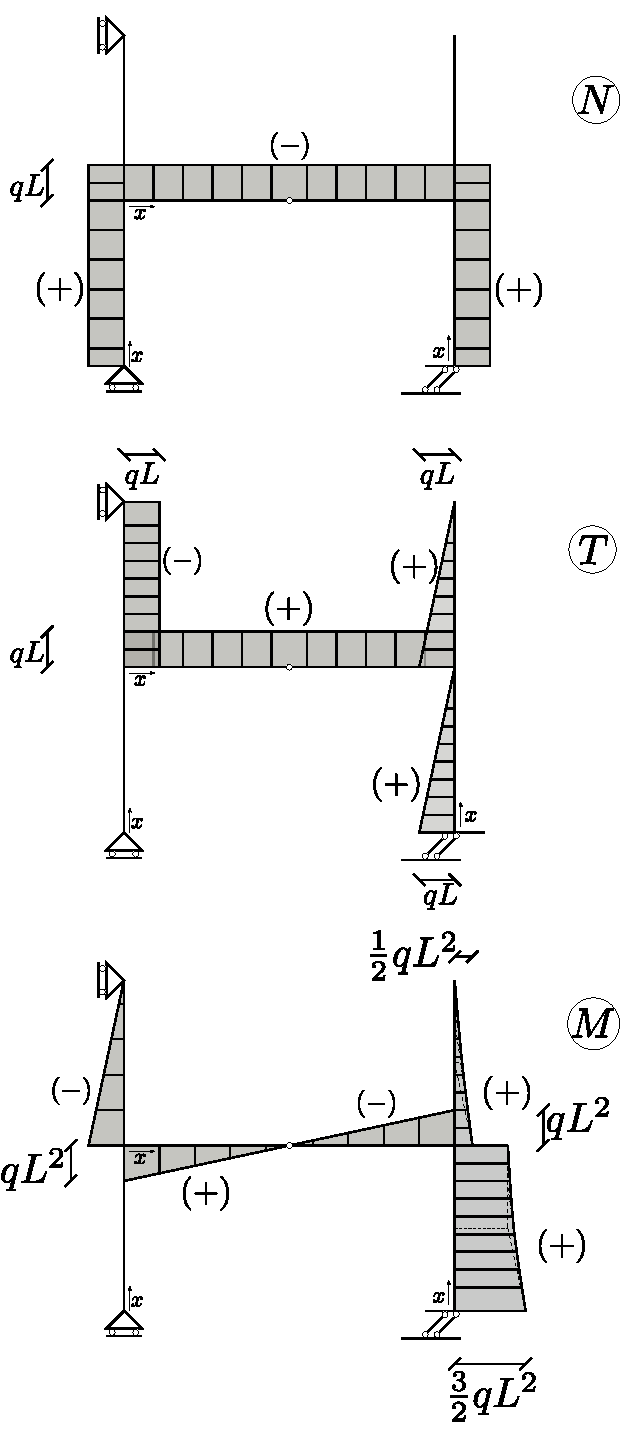
\includegraphics[width=0.58\textwidth]{Immagini/Parte_12/Esercizio12_2/12_2_7.pdf}
\caption{}
\label{Esercizio12-2-7}
\end{figure}
%--------------------------------------------------------------------------------------------------------------------------------------------------------------

%----------------------------------------------------------------------------------------
%----------------------------------------------------------------------------------------
%----------------------------------------------------------------------------------------
%----------------------------------------------------------------------------------------